\documentclass[phd]{ucbthesis}

\usepackage{url}
\usepackage{algorithmic}
\usepackage{algorithm}
\usepackage{listings}
\usepackage{balance}
\usepackage{graphicx}
\usepackage{hyperref}
\usepackage{amsthm}
\usepackage{multirow}
\usepackage{xfrac}

\newtheorem{defn}{Definition}
\newtheorem{lemma}{Lemma}

% \usepackage{draftwatermark}
% \SetWatermarkText{DRAFT}
% \SetWatermarkScale{5}
% "define" Scala
\lstdefinelanguage{scala}{morekeywords={class,object,trait,extends,with,new,if,while,for,def,val,var,this},
otherkeywords={->,=>},
sensitive=true,
morecomment=[l]{//},
morecomment=[s]{/*}{*/},
morestring=[b]"}
% Default settings for code listings
\lstset{frame=tb,language=scala,aboveskip=3mm,belowskip=3mm,showstringspaces=false,columns=flexible,basicstyle={\small\ttfamily}}
\usepackage{amsmath}

\begin{document}

\frontmatter

\title{Scalable Systems and Algorithms for Genomic Variant Analysis}
\author{Frank Austin Nothaft}
\degreesemester{Fall}
\degreeyear{2017}
\degree{Doctor of Philosophy}
\chair{Professor Anthony Joseph}
\cochair{Professor David Patterson}
\othermembers{Professor Haiyan Huang}
\numberofmembers{3}
\field{Computer Science}
\campus{Berkeley}

\maketitle

\approvalpage
\copyrightpage

\begin{abstract}
  With the cost of sequencing a human genome dropping below \$1,000,
  population-scale sequencing has become feasible. With projects that sequence
  more than 10,000 genomes becoming commonplace, there is a strong need for
  genome analysis tools that can scale across distributed computing
  resources while providing reduced analysis cost. Simultaneously, these tools
  must provide programming interfaces and deployment models that are easily
  usable by biologists.

  In this dissertation, we describe the \textsc{ADAM} system for processing
  large genomic datasets using distributed computing. \textsc{ADAM} provides
  a decouped stack-based architecture that can accomodiate many data formats,
  deployment models, and data access patterns. Additionally, \textsc{ADAM}
  defines schemas that describe common genomic datatypes. \textsc{ADAM}'s
  schemas and programming models enable the easy integration of disparate
  genomic datatypes and datasets into a single analysis.

  To validate the \textsc{ADAM} architecture, we implemented an end-to-end
  variant calling pipeline using \textsc{ADAM}'s APIs. To perform parallel
  alignment, we developed the \textsc{Cannoli} tool, which uses \textsc{ADAM}'s
  APIs to automatically parallelize single node aligners. We then
  implemented \textsc{GATK}-style alignment refinement as part of \textsc{ADAM}.
  Finally, we implemented a biallelic genotyping model, and novel reassembly
  algorithms in the \textsc{Avocado} variant caller. This pipeline provides
  state-of-the-art SNV calling accuracy, along with high~(97\%) INDEL calling
  accuracy. To further validate this pipeline, we reanalyzed 270 samples from
  the Simons Genome Diversity Dataset.
\end{abstract}

\tableofcontents

\mainmatter

\part{Introduction and Principles}

\chapter{Introduction}
\label{chap:introduction}

The rapid decrease in sequencing cost has made large scale sequencing
tractible. The dramatic improvement in sequencing cost since the Human
Genome Project has enabled a human whole genome sequence~(WGS) to be
generated for under \$1,000 in wetlab costs~\cite{nhgri}. This trend
will continue for the forseeable future, as sequencing vendors like
Illumina unveil new sequencers such as the NovaSeq that provide even
higher throughput while also decreasing cost, and as radically new
sequencing technologies like Oxford Nanopore come online~\cite{jain17}.
The reduced cost of sequencing enables the use of genome sequencing in
population health research projects and clinical practice. As a result,
the total volume of sequencing data produced is expected to exceed that
of YouTube by 2021~\cite{stephens15}.

The massive scale of the sequencing data this is being acquired enables
novel insight into biological phenomena. The Exome Aggregation
project~\cite{lek16}--now gnomAD--provides an especially powerful
demonstration: by sequencing more than 60,000 exomes, we have been able
to better understand the impact of genomic variation on prion
disease~\cite{minikel16} and cardiovascular disease~\cite{walsh16}, and to
better characterize the effect of structural variation~\cite{ruderfer16}.
However, this scale of data solves biological problems at the cost of techincal
and logistical problems. Data storage and transfer has become a serious problem,
and the focus of many researchers~\cite{fritz11, kozanitis11} and standards
organizations~\cite{paten15}. Not only is the volume of data large, but
expensive processing is needed to analyze the data. Due to historical design
decisions, much of this processing is currently restricted to single node
architectures that assume POSIX storage APIs. As a result, it can take well
upwards of 100 hours to analyze the raw read data from a single genome.

We believe that distributed computing architectures are a good match for
genomic data analysis. Horizontally scalable storage architectures can
simultaneously provide increased data storage capacities, data access
throughput, and reduced storage cost. Because most genomic analyses are centered
on analyzing the genomic data at disparate genomic loci without coordination
betwen loci, most genomic analysis tasks can be executed in parallel. Even more
importantly, these analysis patterns cleanly map onto quasi-relational primitives
that are powerful and can be executed in parallel. Finally, by building upon
widely used open-source distributed processing architectures like \textsc{Apache
Spark}~\cite{zaharia12} and \textsc{Hadoop}~\cite{hadoop}, genomics can benefit
from engineering contributions from a broader swath of engineering.

In this thesis, we introduce \textsc{ADAM}, an application programming
interface~(API) for processing genomic data using Apache Spark. \textsc{ADAM}
is based around a novel stack-oriented architecture that uses schemas to define
the narrow waist in the stack. On top of the schemas, we provide high-level
APIs that allow computational biologists and bioinformaticians to manipulate
collections of genomic data in a parallel fashion. The high level APIs extend
\textsc{Apache Spark}'s Resilient Distributed Dataset~(RDD, see Zahaira et
al.~\cite{zaharia12}) abstraction with genomics-specific functionality, and
eliminates the low level ``walker'' pattern~\cite{mckenna10} that is common in
genomics. At lower levels in the stack, we provide efficient implementations
of the common genomics query models. By having clearly defined APIs between
each level of the stack, we are able to exchange layers to optimize query
performance for a given query, input data type, or cluster/cloud configuration.

Our work on \textsc{ADAM} has resulted in the broad ecosystem of projects
depicted in Figure~\ref{fig:bdg}. We refer to the tools built on \textsc{ADAM}
as the ``Big Data Genomics''~(BDG) project. In this dissertation, we will limit
our focus to \textsc{ADAM}'s architecture and APIs, and the tools and algorithms
that form the core components of the BDG variant calling pipeline:

\begin{itemize}
\item \textsc{Cannoli}, which parallelizes single node genomic data processing
  tools. \textsc{Cannoli} is used in our pipeline for alignment.
\item The \textsc{ADAM} read transformations, which correct for errors in the
  aligned reads.
\item \textsc{Avocado}, a fully parallelized variant caller.
\end{itemize}

This pipeline is able to call variants on a high coverage ($60\times$) whole
genome in under one hour when running on commodity cloud computing resources.
This represents a dramatic improvement in performance over the widely used
Genome Analysis Toolkit~(GATK, see DePristo et al.~\cite{depristo11}), which
needed over 100 hours to call variants on the same sample. These tools
demonstrate how \textsc{ADAM}'s APIs enable bioinformatics analyses to be
written at a high level, while also allowing for the reuse of code from legacy
bioinformatics tools.

\begin{figure}[h]
\begin{center}
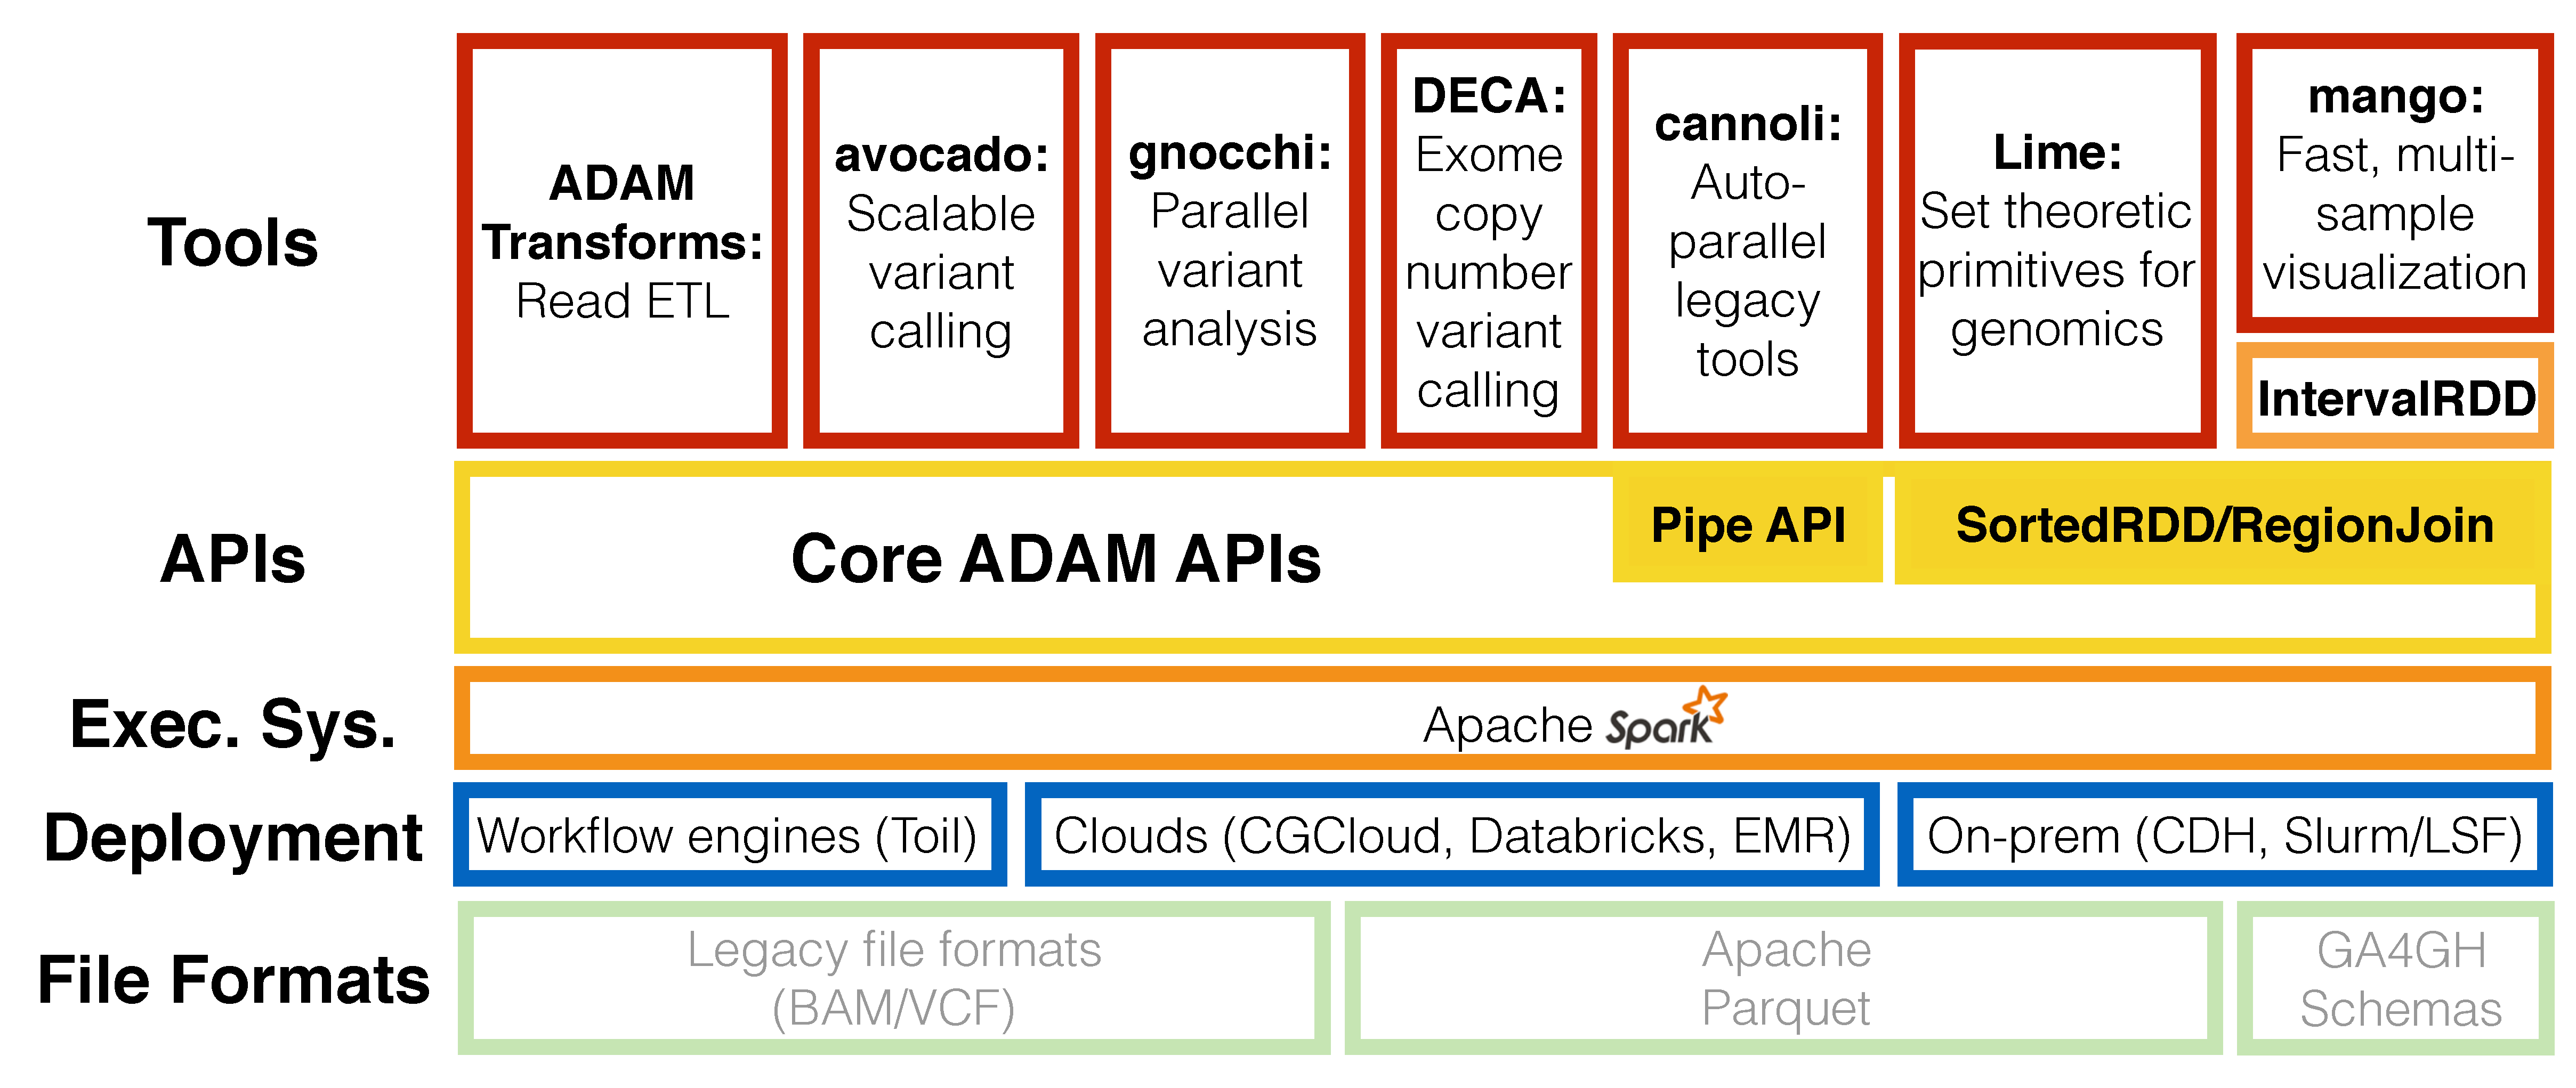
\includegraphics[width=0.95\linewidth]{graphs/bdgenomics-stack.pdf}
\end{center}
\caption{The Big Data Genomics ecosystem. Our work on \textsc{ADAM} has
  built a framework for scalable genomics using external projects like
  \textsc{Apache Spark}~\cite{zaharia12} and \textsc{Apache
  Parquet}~\cite{parquet}. On top of \textsc{ADAM}'s core APIs, we have
  built a broad ecosystem of tools~\cite{tu16, morrow17, linderman17}
  demonstrating how \textsc{Apache Spark} can accelerate genomic data
  analysis. To enable the reproducible use of \textsc{Apache Spark} in
  scientific data analysis workloads, we have contributed to novel,
  cloud-native workflow systems~\cite{vivian17}.}
\label{fig:bdg}
\end{figure}

In this dissertation, we begin by describing the deluge of genomic data and the
tools that are used to process, manipulate, and store genomic data. In part two,
we then describe the requirements for a distributed genomic data analysis
framework and introduce \textsc{ADAM}'s architecture. Part three describes how
we built the \textsc{Cannoli}-\textsc{ADAM}-\textsc{Avocado} variant calling
pipeline on top of \textsc{ADAM}'s architecture, and the novel algorithms and
architectural refinements that were needed. We then validate the accuracy of
this pipeline in part four using ground truth datasets~\cite{zook15} and a large
scale sequencing project~\cite{mallick16}. We conclude by describing open
problems and future directions for this research, as well as the impact of the
Big Data Genomics/\textsc{ADAM} project.

\section{Economic Trends and Population Scale Sequencing}
\label{sec:economic-trends-population-scale}

\begin{itemize}
\item Genomic data is often only meaningful when viewed in aggregate.
  \begin{itemize}
  \item The association between genotype and phenotype is often weak, unless
    the variant under study is strongly pathogenic.
  \item Many diseases are not driven by a single genotype, but rather by the
    combined effect of multiple genotypes.
  \item For example, in AML there is a spread spectrum of mutations which
    fall into several clearly distinct disease subtypes. What is the impact of
    a single mutation?
  \end{itemize}
\item Technical innovation has made large scale sequencing tractible.
  \begin{itemize}
  \item NHGRI ``Moore's Law'' plot.
  \item While the sequencing technology used in the Human Genome Project was
    expensive, current whole genome sequencing technology is inexpensive.
  \item Additionally, exome and targeted capture techniques can further reduce
    costs.
  \end{itemize}
\item Population scale sequencing projects are no longer unprecidented.
  \begin{itemize}
  \item The 1,000 Genomes project is now small data; there are a multitude of
    projects that have sequenced at the 10,000+ sample scale.
  \item These include the UK10K, Exome Aggregation Consortium, and Genomics
    England, among others.
  \end{itemize}
\item Finally, large scale sequencing projects are moving out of research and
  into practice.
  \begin{itemize}
  \item Large scale sequencing projects can inform both drug design and risk
    models.
  \item GSK/NHS public/private model for Genomics England
  \item Modeling risk via sequencing for cancer at Color Genomics
  \item Regeneron/Geisenger tie-up
  \end{itemize}
\end{itemize}

\section{The Case for Distributed Computing for Genomic Analysis}
\label{sec:distributed-computing-for-genomics}

\begin{itemize}
\item Most genomic analysis tasks map naturally to distributed computing.
  \begin{itemize}
  \item Heavyweight analyses either typically work on unaligned data, or on
    a sorted stream across aligned data.
  \item These patterns typically can be parallelized without significant
    communication.
  \item Additionally, there are many queries that map directly onto
    relational primitives.
  \end{itemize}
\item We believe we need to clean slate re-architect genomics for distributed
  computing.
  \begin{itemize}
  \item Genomics tools are typically designed assuming a flattened stack running
    on a single node, or on a HPC-style cluster.
  \item There have been several attempts to retrofit tools onto distributed
    computing, e.g., \textsc{CloudBurst}/\textsc{Crossbow} using Hadoop
    Streaming.
  \item There have been several attempts to retrofit genomics specific file
    formats onto distributed query architectures, e.g., \textsc{SegPig},
    \textsc{BioPig}.
  \item However, these implementations provide either poor programming costs or
    inefficient and limited query mechanisms.
  \item By doing a clean-slate rearchitecture, we can eliminate architectural
    problems and provide better user-facing query models with better performance.
  \end{itemize}
\end{itemize}

\section{Mapping Genomics onto Distributed Computing using \textsc{ADAM}}
\label{sec:mapping-genomics-to-distributed-computing}

\begin{itemize}
\item To this end, we propose \textsc{ADAM}.
  \begin{itemize}
  \item Define schemas for genomic datatypes, which provide data independence.
  \item These schemas form the basis of a narrow waisted stack, which yields
    APIs that support both genomic query and metadata management, and which can
    be used across multiple languages.
  \item We implement this architecture on top of \textsc{Apache Spark}, one of
    the most widely used distributed computing frameworks.
  \end{itemize}
\item To demonstrate \textsc{ADAM}, we have built an end-to-end variant calling
  pipeline.
  \begin{itemize}
  \item This pipeline includes distributed implementations of alignment, read
    preprocessing, and variant calling.
  \item The pipeline can run end-to-end on a $60\times$ coverage whole genome
    in under an hour, at a cost of $<$\$15 on cloud computing.
  \item This pipeline provides results comparable to state of the art for SNV
    calling, and high accuracy (97\%) for INDEL calling.
  \end{itemize}
\item \textsc{ADAM} improves over conventional genomics tools by providing:
  \begin{itemize}
  \item Schemas which can support loading data from a large variety of formats.
  \item High level, quasi-relational APIs for manipulating genomic data in both
    single node and cluster environments.
  \item Parallel I/O across genomics file formats.
  \item A simple API for parallelizing single node genomic tools with a minimal
    amount of code.
  \end{itemize}
\item \textsc{ADAM} has enabled a large ecosystem of work
\end{itemize}

\chapter{Background and Related Work}
\label{chap:background}

\begin{itemize}
\item This dissertation focuses on the ``genome resequencing'' pipeline.
  \begin{itemize}
  \item I.e., given a known genome assembly, identify the edits between this
    individual and the assembly.
  \item We assume short reads.
  \item 
  \end{itemize}
\end{itemize}

\section{Genome Sequencing Technologies}
\label{sec:genome-sequencing}

\begin{itemize}
\item How are reads sequenced?
  \begin{itemize}
  \item Illumina uses a sequencing-by-synthesis approach.
  \item Dyes are attached to nucleotides.
  \item The dyes are imaged, washed off, and new dyes are attached.
  \item Image to go here.
  \end{itemize}
\item Where does the DNA come from?
  \begin{itemize}
  \item Sample prep and extraction...
  \item Details to be added, depending on amount of detail suggested.
  \end{itemize}
\item Data characteristics:
  \begin{itemize}
  \item Relative error rates, bias patterns, etc...
  \item Differences between whole genome, whole exome.
  \end{itemize}
\end{itemize}

\section{Genomic Analysis Tools and Architectures}
\label{sec:genomic-analysis}

\subsection{Genomic Data Representations}
\label{sec:genomic-data-representations}

\begin{itemize}
\item Widely used formats were developed mostly during the 1,000 Genomes
  project.
  \begin{itemize}
  \item The \textsc{Sequence Alignment/Mapping}~(SAM) format was developed as
    a way to represent genomic reads.
  \item The \textsc{Variant Call Format}~(VCF) format was defined to store
    variants and genotypes.
  \item Both are tab delimited text file formats that store semistructured data.
  \end{itemize}
\item These formats begat later binary versions that provide improved
  compression and performance.
  \begin{itemize}
  \item SAM/VCF were supplanted by binary variants (BAM/BCF)
  \item Additionally, there was significant interest in compressed storage
    formats for genomic data (most significantly, CRAM)
  \end{itemize}
\item Schemas for representing genomic data:
  \begin{itemize}
  \item GA4GH APIs
  \item OpenCB APIs
  \end{itemize}
\end{itemize}

\subsection{Genomic Analysis Architectures}
\label{sec:genomic-architectures}

\begin{itemize}
\item The main genomic analysis architecture out there is the GATK.
  \begin{itemize}
  \item Uses an iterator-based model called a ``walker'' to traverse over
    data aligned to reference genome coordinates.
  \item Puports a map-reduce style API, but historically only provided single
    node execution (multithreaded).
  \item Multi-node execution was provided through the Queue workflow manager.
  \item Revisit this in the context of the GATK4.
  \end{itemize}
\item Several alternative approaches have included the Google Genomics and
  OpenCB approaches.
  \begin{itemize}
    \item Google Genomics is built heavily on top of BigQuery.
  \end{itemize}
\item Workflow management as an alternate paradigm?
  \begin{itemize}
  \item How much can genomics be ``parallel-by-sample''?
  \item See GATK Queue.
  \item Toil, Cromwell, CWL, WDL, NextFlow...
  \end{itemize}
\end{itemize}

\subsection{Variant Calling Approaches}
\label{sec:variant-calling-approaches}


The accuracy of insertion and deletion~(INDEL) variant discovery has been improved by the development
of variant callers that couple local reassembly with haplotype-based statistical models to recover INDELs
that were locally misaligned~\cite{albers11}. Now, several prominent variant callers such as the Genome
Analysis Toolkit's~(GATK) \textsc{HaplotypeCaller}~\cite{depristo11}, \textsc{Scalpel}~\cite{narzisi14}, and
\textsc{Platypus}~\cite{rimmer14}. Although haplotype-based methods have enabled more accurate INDEL
and single nucleotide polymorphism~(SNP) calls~\cite{bao14}, this accuracy comes at the cost of
end-to-end runtime~\cite{talwalkar14}. Several recent projects have been focused on improving
reassembly cost either by limiting the percentage of the genome that is reassembled~\cite{bloniarz14} or
by improving the performance of the core algorithms used in local reassembly~\cite{rimmer14}.

The performance issues seen in haplotype reassembly approaches derives from the high asymptotic
complexity of reassembly algorithms. Although specific implementations may vary slightly, a typical
local reassembler performs the following steps:

\begin{enumerate}
\item A de Bruijn graph is constructed from the reads aligned to a region of the reference genome,
\item All valid paths~(\emph{haplotypes}) between the start and end of the graph are enumerated,
\item Each read is realigned to each haplotype, typically using a pair Hidden Markov Model~(HMM,
see Durbin et al~\cite{durbin98}),
\item A statistical model uses the read$\leftrightarrow$haplotype alignments to choose the haplotype pair
that most likely represents the variants hypothesized to exist in the region, 
\item The alignments of the reads to the chosen haplotype pair are used to generate statistics that are
then used for genotyping.
\end{enumerate}

In this paper, we focus on improving the algorithmic efficiency steps one through three of the local reassembly problem.
We do not focus algorithmically on accelerating stages four and five, as there is wide
variation in the algorithms used in stages four and five. However, we do provide an parallel
implementation of a widely used statistical model for genotyping~\cite{li11}. Stage one (graph
creation) has approximately $\mathcal{O}(r l_r)$ time complexity, and stage two (graph elaboration) has
$\mathcal{O}(h \max(l_h))$ time complexity.
The asymptotic time cost bound of local reassembly comes from stage three, where cost is $\mathcal{O}(h r l_r
\max(l_h))$, where $h$ is the number of haplotypes tested in this region\footnote{The number of
haplotypes tested may be lower than the number of haplotypes reassembled. Several tools
(see Depristo et al~\cite{depristo11} and Garrison and Marth~\cite{garrison12}) allow users to limit the number of haplotypes evaluated to improve
performance.}, $r$ is the number of reads aligned to this region, $l_r$ is the read length\footnote{For
simplicity, we assume constant read length. This is a reasonable assumption as many of the variant
callers discussed target Illumina reads that have constant length.}, and $\min(l_h)$ is the length of the
shortest haplotype that we are evaluating. This complexity comes from realigning $r$ reads to $h$
haplotypes, where realignment has complexity $\mathcal{O}(l_r l_h)$.

In this paper, we introduce the indexed de Bruijn graph and demonstrate how it can be used to
reduce the asymptotic complexity of reassembly. An indexed de Bruijn graph is identical to a
traditional de Bruijn graph, with one modification: when we create the graph, we annotate each
$k$-mer with the index position of that $k$-mer in the sequence it was observed in. This simple addition
enables the use of the indexed de Bruijn graph for $\Omega(n)$ local sequence alignment with
canonical edit representations for most edits. This structure can be used for both sequence alignment and
assembly, and achieves a more efficient approach for variant discovery via local reassembly.
To further improve the efficiency of this approach, we demonstrate in~\S\ref{sec:implementation}
how we can implement the canonicalization scheme that we demonstrate using indexed de Bruijn
graphs without constructing a de Bruijn graph that contains both sequences.

Current variant calling pipelines depend heavily on realignment based approaches for accurate
genotyping~\cite{li14}. Although there are several approaches that do not make explicit use of reassembly,
all realignment based variant callers use an algorithmic structure similar to the one described
above. In non-assembly approaches like \textsc{FreeBayes}~\cite{garrison12}, stages
one and two are replaced with a single step where the variants observed in the reads aligned to a given
haplotyping region are filtered for quality and integrated directly into the reference haplotype in that region.
In both approaches, local alignment errors~(errors in alignment \emph{within} this region) are corrected
by using a statistical model to identify the most likely location that the read could have come from, given
the other reads seen in this area.

Although the model used for choosing the best haplotype pair to finalize realignments to varies between
methods~(e.g., the GATK's \textsc{IndelRealigner} uses a simple log-odds model~\cite{depristo11}, while
methods like \textsc{FreeBayes}~\cite{garrison12} and \textsc{Platypus}~\cite{rimmer14} make use of richer
Bayesian models), these methods require an all-pairs alignment of reads to candidate
haplotypes. This leads to the runtime complexity bound of $\mathcal{O}(h r l_r \min(l_h))$,
as we must realign $r$ reads to $h$ haplotypes, where the cost of realigning
one read to one haplotype is $\mathcal{O}(l_r \max(l_h))$, where $l_r$ is the read length~(assumed to be
constant for Illumina sequencing data) and $\max(l_h)$ is the length of the longest haplotype. Typically,
the data structures used for realignment~($\mathcal{O}(l_r \max(l_h))$ storage cost) can be reused.
These methods typically retain \emph{only} the best local realignment per read per haplotype, thus
bounding storage cost at $\mathcal{O}(h r)$.

For non-reassembly based approaches, the cost of generating candidate haplotypes is $\mathcal{O}(r)$,
as each read must be scanned for variants, using the pre-existing alignment. These variants are typically
extracted from the CIGAR string, but may need to be normalized~\cite{li14}. de Bruijn graph based 
reassembly methods have similar $\mathcal{O}(r)$ time complexity for building the de Bruijn
graph as each read must be sequentially broken into $k$-mers, but these methods have a different
storage cost. Specifically, storage cost for a de Bruijn graph is similar to $\mathcal{O}(k
(l_{\text{ref}} + l_{\text{variants}} + l_{\text{errors}}))$, where $l_{\text{ref}}$ is the length of the reference
haplotype in this region, $l_{\text{variants}}$ is the length of true variant sequence in this region, 
$l_{\text{errors}}$ is the length of erroneous sequence in this region, and $k$ is the $k$-mer size. In
practice, we can approximate both errors and variants as being random, which gives $\mathcal{O}(k
l_{\text{ref}})$ storage complexity. From this graph, we must enumerate the haplotypes present in the
graph. Starting from the first $k$-mer in the reference sequence for this region, we perform a depth-first
search to identify all paths to the last $k$-mer in the reference sequence. Assuming that the graph is
acyclic~(a common restriction for local assembly), we can
bound the best case cost of this search at $\Omega(h \min l_h)$.

The number of haplotypes evaluated, $h$, is an important contributor to the algorithmic complexity of
reassembly pipelines, as it sets the storage and time complexity of the realignment scoring phase, the
time complexity of the haplotype enumeration phase, and is related to the storage complexity of the
de Bruijn graph. The best study of the complexity of assembly techniques was done by Kingsford
et al.~\cite{kingsford10}, but is focused on \emph{de novo} assembly and pays special attention to
resolving repeat structure. In the local realignment case, the number of haplotypes identified is determined
by the number of putative variants seen. We can na\"{i}vely model this cost with \eqref{eq:haplotypes},
where $f_v$ is the frequency with which variants occur, $\epsilon$ is the rate at which bases are
sequenced erroneously, and $c$ is the coverage (read depth) of the region.

\begin{align}
\label{eq:haplotypes}
h \sim f_v l_{\text{ref}} + \epsilon l_{\text{ref}} c
\end{align}

This model is na\"{i}ve, as the coverage depth and rate of variation varies across sequenced datasets,
especially for targeted sequencing runs~\cite{fang14}. Additionally, while the $\epsilon$ term models the
total number of sequence errors, this is not completely correlated with the number of \emph{unique}
sequencing errors, as sequencing errors are correlated with sequence context~\cite{depristo11}. Many
current tools allow users to limit the total number of evaluated haplotypes, or apply strategies to minimize
the number of haplotypes considered, such as filtering observed variants that are likely to be sequencing
errors~\cite{garrison12}, restricting realignment to INDELs~(\textsc{IndelRealigner},~\cite{depristo11}), or
by trimming paths from the assembly graph. Additionally, in a de Bruijn graph, errors in the
first $k$ or last $k$ bases of a read will manifest as spurs and will not contribute paths through the graph. We provide~\eqref{eq:haplotypes} solely as a motivating
approximation, and hope to study these characteristics in more detail in future work.

\section{Distributed Computing Platforms}
\label{sec:distributed-computing}

\subsection{Distributed Genomic Analysis Tools}
\label{sec:distributed-genome-analysis}

\begin{itemize}
\item Tools retrofitted on top of distributed computing:
  \begin{itemize}
  \item CloudBurst
  \item CrossBow
  \item CloudScale-BWAMem
  \item Halvalde
  \end{itemize}
\item Genomics tools designed for distributed computing:
  \begin{itemize}
  \item SparkSeq
  \item VariantSpark    
  \item Query models for Genomics on distributed computing: SeqPig, BioPig
  \item OpenCB
  \item GATK4
  \item Hail
  \end{itemize}
\item Genome assembly and HPC architectures:
  \begin{itemize}
  \item Won't discuss much in this paper, but genome assembly has different
    access patterns, more amenable to HPC
  \item AbYSS on MPI
  \item PGAS approaches to de Bruijn graph traversal
  \end{itemize}
\end{itemize}

\part{Architecture and Infrastructure}

\chapter{Design Principles for Scalable Genomics}
\label{chap:design}

\begin{itemize}
\item Initially, \textsc{ADAM} had several goals:
  \begin{itemize}
  \item Provide clean APIs for writing large scale genomic data analyses
  \item Raise abstraction by centering data manipulation around schemas instead
    of file formats
  \item Allow these APIs to be exposed across commonly used languages
  \end{itemize}
\item To do this, \textsc{ADAM} used a decoupled, stack-oriented architecture
\item Over time, these goals grew in scope to include:
  \begin{itemize}
  \item Support coordinate-space joins with genomic data
  \item Support exploratory data analysis on genomic datasets
  \item Allow people to reuse their existing genomic analysis tools on Spark with
    minimal modifications
  \end{itemize}
\item Supporting these goals was enabled by \textsc{ADAM}'s decoupled architecture
\end{itemize}

\section{A Stack Architecture for Scientific Data Processing}
\label{sec:stack-architecture}

The processing patterns being applied to scientific data shift widely as the data itself ages. Because of
this change, we want to design a scientific data processing system that is flexible enough to
accommodate our different use cases. At the same time, we want to ensure that the components in the
system are well isolated so that we avoid bleeding functionality across the stack. If we bleed functionality
across layers in the stack, we make it more difficult to adapt our stack to different applications.
Additionally, as we discuss in~\S\ref{sec:read-preprocessing}, improper separation of concerns can
actually lead to errors in our application.

These concerns are very similar to the factors that led to the development of the Open Systems
Interconnection~(OSI) model and Internet Protocol~(IP) stack for networking
services~\cite{zimmermann80}. The networking stack models were designed to allow the mixing and
matching of different protocols, all of which existed at different functional levels. The success of the
networking stack model can largely be attributed to the ``narrow waist'' of the stack, which simplified the
integration of a new protocol or technology by ensuring that the protocol only needed to implement a
single interface to be compatible with the rest of the stack.

Unlike conventional scientific systems that leverage custom data formats like BAM or SAM~\cite{li09},
or CRAM~\cite{fritz11}, we believe that the use of an explicit schema for data interchange is critical.
In our stack model shown in Figure~\ref{fig:stack-model}, the schema becomes the ``narrow waist''
of the stack. Most importantly, placing the schema as the narrow waist enforces a strict separation
between data storage/access and data processing. Additionally, this enables literate programming
techniques which can clarify the data model and access patterns. The seven layers of our stack model
are decomposed as follows, and are numbered in ascending order from bottom to top:

\begin{enumerate}
\item \textbf{Physical Storage:} This layer coordinates data writes to physical media.
\item \textbf{Data Distribution:} This layer manages access, replication, and distribution of the files that have
been written to storage media.
\item \textbf{Materialized Data:} This layer encodes the patterns for how data is encoded and stored. This
layer determines I/O bandwidth and compression.
\item \textbf{Data Schema:} This layer specifies the representation of data, and forms the narrow waist of
the stack that separates access from execution.
\item \textbf{Evidence Access:} This layer provides us with primitives for processing data, and allows us to
transform data into different views and traversals.
\item \textbf{Presentation:} This layer enhances the data schema with convenience methods for performing
common tasks and accessing common derived fields from a single element.
\item \textbf{Application:} At this level, we can use our evidence access and presentation layers to compose
the algorithms to perform our desired analysis.
\end{enumerate}

A well defined software stack has several other significant advantages. By limiting application
interactions with layers lower than the presentation layer, application developers are given a clear and
consistent view of the data they are processing, and this view of the data is independent of whether the
data is local or distributed across a cluster or cloud. By separating the API from the data access layer,
we improve flexibility. With careful design in the data format and data access layers, we can seamlessly
support conventional whole file access patterns, while also allowing easy access to small slices of files.
By treating the compute substrate and storage as separate layers, we also drastically increase
the portability of the APIs that we implement.

As we discuss in more detail in~\S\ref{sec:read-preprocessing}, current scientific systems bleed
functionality between stack layers. An exemplar is the SAM/BAM and CRAM formats, which expect data
to be sorted by genomic coordinate. This order modifies the layout of data on disk~(level 3, Materialized Data)
and constrains how applications traverse datasets~(level 5, Evidence Access). Beyond
constraining applications, this leads to bugs in applications that are difficult to detect.\footnote{The
current best-practice implementations of the BQSR and Duplicate Marking algorithms both fail when
processing certain corner-case alignments. These errors are caused because of the requirement to
traverse reads in sorted order.} These views of evidence should be implemented at the evidence
access layer instead of in the layout of data on disk. This split enforces independence of anything below the
schema.

The idea of decomposing scientific applications into a stack model is not new; Bafna et al~\cite{bafna13}
made a similar suggestion in 2013. We borrow some vocabulary from Bafna et al, but our approach is
differentiated in several critical ways:

\begin{itemize}
\item Bafna et al consider the stack model specifically in the context of data management systems for
genomics; as a result, they bake current technologies and design patterns into the stack. In our opinion,
a stack design should serve to abstract layers from methodologies/implementations. If not, future
technology trends may obsolete a layer of the stack and render the stack irrelevant.
\item Bafna et al define a binary data format as the narrow waist in their stack, instead of a schema.
While these two seem interchangeable, they are not in practice. A schema is a higher level of abstraction
that encourages the use of literate programming techniques and allows for data serialization techniques
to be changed as long as the same schema is still provided.
\item Notably, Bafna et al use this stack model to motivate GQL~\cite{kozanitis14}. While a query system
should provide a way to process and transform data, Bafna et al instead move this system down to the
data materialization layer. We feel that this inverts the semantics that a user of the system would prefer
and makes the system less general.
\end{itemize}

Deep stacks like the OSI stack~\cite{zimmermann80} are generally simplified for practical use. Conceptually,
the stack we propose is no exception. In practice, we combine layers one and two, and layers five and six.
There are several reasons for these mergers. First, in \texttt{Hadoop}-based systems, the system does not have practical visibility
below layer two, thus there is no reason to split layers one and two except as a philosophical exercise.
Layers five and six are commingled because some of the enriched presentation objects are used to
implement functionality in the evidence access layer. This normally happens when a key is needed, such as
when repartitioning the dataset, or when reducing or grouping values.

\chapter{The \textsc{ADAM} Architecture}
\label{chap:architecture}

Due to both the growing volume of genomic sequencing data and the large size of these datasets,
sequencing centers face the increasingly difficult task of turning around genomic data analyses in a
reasonable timeframe~\cite{schadt10, stein10}. While the per-run latency of current genomic pipelines
such as the \texttt{GATK} can be improved by manually partitioning the input dataset and distributing
work, native support for distributed computing is not provided. As a stopgap solution, projects like
\texttt{Cloudburst}~\cite{schatz09} and \texttt{Crossbow}~\cite{langmead09} have ported individual
analytics tools to run on top of \texttt{Hadoop}. While this approach has served well for proofs of concept,
it provides poor abstractions for application developers and makes it difficult to create novel distributed
genomic analyses, and does little to attack sources of inefficiency or incorrectness in distributed
genomics pipelines.

To address these problems, we need to reconsider how to build software for processing genomic data.
Modern genome analysis pipelines are built around monolithic architectures and flat file formats.
These architectures are designed to efficiently run current algorithms on single node processing
systems, but impose significant restrictions. These restrictions include:

\begin{itemize}
\item These implementations are locked to a single node processing model. Even the \texttt{GATK}'s
``map-reduce'' styled \texttt{walker} API~\cite{mckenna10} is limited to natively support processing on
a single node. While these jobs can be manually partitioned and run in a distributed setting, manual
partitioning can lead to imbalance in work distribution and makes it difficult to run algorithms that
require aggregating data across all partitions, and lacks the fault tolerance provided by modern
distributed systems such as \texttt{Hadoop} or \texttt{Spark}~\cite{zaharia12}.
\item Most of these implementations \emph{assume} invariants about the sorted order of records on
disk. This ``stack smashing'' (specifically, the layout of data is used to ``accelerate'' a processing stage)
can lead to bugs when data does not cleanly map to the assumed sort order. Additionally, since these
sort order invariants are rarely explicit and vary from tool to tool, pipelines assembled from disparate
tools can be brittle. We discuss this more in~\S\ref{sec:read-preprocessing} and footnote 1.
\item Additionally, while these invariants are intended to improve performance, it is not clear that these
invariants \emph{actually} improve performance. There are two common sort invariants used in genomics:
sort by reference position and sort by read name. Changing between these two sort orders entails
a full shuffle and resort of the dataset. Additionally, a sort is required after alignment to establish a sort order.
\end{itemize}

As noted above, current implementations are locked to a single node model. Projects like
\texttt{Hadoop-BAM}~\cite{niemenmaa12}, \texttt{SeqPig}~\cite{schumacher14}, and \texttt{BioPig}~\cite{nordberg13}
have attempted to build a distributed processing environment on top of current single node genomics APIs.
However, several problems must be solved in order to make distributed processing of genomic data productive:

\begin{itemize}
\item Current genomics data formats rely on a centralized header for storing experiment metadata. Since the
metadata is centralized, it must be replicated to all machines.
\item A simple map-reduce or SQL-like API is insufficient for implementing genomic analyses. Rather, to enhance
bioinformatician productivity, we need to define APIs that allow developers to conveniently express algorithms.
\end{itemize}

In \texttt{ADAM}, we have taken a more aggressive approach to the design of APIs for processing genomic data
in a distributed system. Although modern genomics pipelines are built as monolithic applications, we have
chosen a layered decomposition for \texttt{ADAM}, that uses a schema as a ``narrow waist''. Instead of using
a flat file format, as is traditional in genomics, we are using this schema with \texttt{Parquet}~(a commodity columnar
store~\cite{parquet}) to store genomic data in a way that both allows efficient distributed read/write and that
achieves high compression. On top of this, we have added primitives that implement common genomic traversals
in a distributed manner. We have then used \texttt{ADAM} to implement common preprocessing stages from
commonly used genomics pipelines. \texttt{ADAM}'s preprocessing stages are between 1-5$\times$ faster than the
equivalent \texttt{GATK} preprocessing stages, and achieve linear scaling out to 128 nodes.

\section{Realizing A Decoupled Stack Architecture In \textsc{ADAM}}
\label{sec:realizing-stack-architecture}

\begin{itemize}
\item Implementing a stack architecture requires careful API design
  \begin{itemize}
  \item If APIs are too strictly specified, stack layers can't actually be exchanged
  \item If APIs are too vaguely specified, system is unreliable
  \end{itemize}
\item \textsc{ADAM} ultimately extends two important APIs:
  \begin{itemize}
  \item The \textsc{ADAMContext}: the entrypoint to loading all data
  \item The \textsc{GenomicRDD} abstraction: a wrapper for genomic datasets
  \end{itemize}
\item How are these APIs important in realizing the stack vision?
  \begin{itemize}
  \item Layers 1 and 2 are largely deferred to Apache Spark
  \item Layer 3 is essentially a view; the \textsc{ADAMContext} provides the view
    on load, \textsc{GenomicRDD} provides the view on save
  \item Layer 4 is enclosed in the \textsc{GenomicRDD}
  \item Layers 5 and 6 are implemented in the \textsc{GenomicRDD}; users can
    specialize a \textsc{GenomicRDD} for their specific application/query pattern
  \item Layer 7 is where the user builds their code, and this is built by
    using the \textsc{ADAMContext} to load in a \textsc{GenomicRDD}, which is then
    transformed and saved.
  \end{itemize}
\end{itemize}

\section{Query Patterns for Genomic Data Analysis}
\label{sec:query-patterns}

There are a wide array of experimental techniques and platforms in genome informatics, but many of these
methods produce datapoints that are tied to locations in the genome through the use of genomic coordinates.
Each cell contains a copy of the genome with one molecule per chromosome. Each molecule is a collection of
DNA polymers coated with (and wrapped around) proteins and packed into the nucleus in a complex
3-dimensional shape. In practice, computational biologists abstract this complexity by storing a single long
string that represents the nucleotides of the chromosome. We can then connect a datapoint or observation to the
genome by associating the data with the chromosome name and a point or interval on a 1-dimensional space.

A platform for scientific data processing in genomics needs to understand these 1-dimensional coordinate
systems because these become the basis on which data processing is parallelized. For example, when calling
variants from sequencing data, the sequence data that is localized to a single genomic region (or ``locus'') can be 
processed independently from the data localized to a different region, as long as the regions are far enough
apart.

Beyond parallelization, many of the core algorithms and methods for data aggregation in genomics are phrased
in terms of geometric primitives on 1-D intervals and points where we compute distance, overlap, and
containment.  An algorithm for calculating quality control metrics may try to calculate ``coverage,'' a count
of how many reads overlap each base in the genome. A method for filtering and annotating potential variants
might assess the validity of a variant using the quality characteristics of all reads that overlap the putative variant.

To support these algorithms, we provide a ``region'' or ``spatial'' join primitive. The algorithm used is described
in algorithm~\ref{alg:region-join} and takes as input two sets (RDDs, see Zaharia et al~\cite{zaharia12}) of
\texttt{ReferenceRegions}, a data structure that represents intervals along the 1-D genomics coordinate
space. It produces the set of all overlapping \texttt{ReferenceRegion} pairs. The $hulls$ variable contains
the set of convex hulls and is broadcasted to all compute nodes during the join.

\begin{algorithm}
\caption{Partition And Join Regions via Broadcast}
\label{alg:region-join}
\begin{algorithmic}
\STATE $left \leftarrow$ input dataset; left side of join
\STATE $right \leftarrow$ input dataset; right side of join
\STATE $regions \leftarrow left$.map($data \Rightarrow $generateRegion($data$))
\STATE $regions \leftarrow regions$.groupBy($region \Rightarrow region$.$name$)
\STATE $hulls \leftarrow regions$.findConvexHull()
\STATE $hulls$.broadcast()
\STATE $keyLeft \leftarrow left$.keyBy($data \Rightarrow $getHullId($data$, $hulls$))
\STATE $keyRight \leftarrow right$.keyBy($data \Rightarrow $getHullId($data$, $hulls$))
\STATE $joined \leftarrow keyLeft$.join($keyRight$)
\STATE $truePositives \leftarrow joined$.filter($r1, r2 \Rightarrow r1$.overlaps($r2$))
\RETURN $truePositives$
\end{algorithmic}
\end{algorithm}

To find the maximal set of non-overlapping regions, we must find the convex hull of all regions emitted.
We present a distributed algorithm for finding convex hulls in Appendix \ref{sec:convex-hull}. The
distributed convex hull computation problem is important because it is used both for computing regions
for partitioning during a region join and for performing INDEL realignment.

While the join described above is a broadcast join, a region join can also be implemented via a straightforward
shuffle-based approach, which is described in Algorithm~\ref{alg:shuffle-region-join}. The \texttt{partitionJoinFn}
function maintains two iterators (one each from both the left and right collections), along with a buffer. This buffer is
used to track all key-value pairs from the right collection iterator that \emph{could} match to a future key-value pair
from the left collection iterator. We prune this buffer every time that we advance the left collection iterator. For
simplicity, the description of Algorithm~\ref{alg:shuffle-region-join} ignores the complexity of processing keys that cross
partition boundaries. In our implementation, we replicate keys that cross partition boundaries into both partitions.

\begin{algorithm}
\caption{Partition And Join Regions via Shuffle}
\label{alg:shuffle-region-join}
\begin{algorithmic}
\STATE $left \leftarrow$ input dataset; left side of join
\STATE $right \leftarrow$ input dataset; right side of join
\STATE $partitions \leftarrow left$.getPartitions()
\STATE $left \leftarrow left$.repartitionAndSort($partitions$)
\STATE $right \leftarrow right$.repartitionAndSort($partitions$)
\STATE $joined \leftarrow left$.zipPartitions($right$, \texttt{partitionJoinFn})
\RETURN $joined$
\end{algorithmic}
\end{algorithm}

These joins serve as a core that we can use to build other abstractions with. For example, self-region joins and
multi-region joins are common in genomics, and can be easily implemented using the above implementations.
We are currently working to implement further parallel spatial functions such as sliding windows, using techniques
similar to the shuffle-based join. We are working to characterize the performance differences between the two
join strategies described above. In the future, we hope to enable the use of the region join in a SQL based system
such as \texttt{Spark SQL}~\cite{armbrust15}.

\section{Schema Design for Representing Genomic Data}
\label{sec:schema-design}

A common criticism of bioinformatics as a field surrounds the proliferation of file formats. Short read data alone is
stored in four common formats: \texttt{FASTQ}~\cite{cock10}, \texttt{SAM}~\cite{li09}, \texttt{BAM}, and
\texttt{CRAM}~\cite{fritz11}. While these formats all represent different layouts of data on disk, they tend to be
logically harmonious. Due to this logical congruency of the different formats, we chose to build \texttt{ADAM}
on top of a logical schema, instead of a binary format on disk. While we do use Apache \texttt{Parquet}~\cite{parquet} to
materialize data on disk, the Apache \texttt{Avro}~\cite{avro} schema is used as a narrow waist in the system,
that enables ``legacy'' formats to be processed identically to data stored in \texttt{Parquet} with modest performance
degradation.

We made several high level choices when designing the schemas used in \texttt{ADAM}. First, the schemas are fully
denormalized, which reduces the cost of metadata access and simplifies metadata distribution. We are able to
get these benefits without greatly increasing the cost of memory access because our backing store~(\texttt{Parquet})
makes use of run length and dictionary encoding, which allows for a single object to be allocated for highly repetitive
elements on read. Another key design choice was to require that all fields in the schema are nullable; by enforcing
this requirement, we enable arbitrary user specified projections. Arbitrary projections can be used to accelerate
common sequence quality control algorithms such as Flagstat~\cite{massie13, nothaft15}.

We have reproduced the schemas used to describe reads, variants, and genotypes below. \texttt{ADAM} also
contains schemas for describing assembled contigs, genomic features, and variant annotations, but we have
not included them in this section.

\begin{lstlisting}[caption=\texttt{ADAM} read schema]
record AlignmentRecord {
  /** Alignment position and quality */
  Contig contig;
  long start;
  long oldPosition;
  long end;

  /** read ID, sequence, and quality */
  string readName;
  string sequence;
  string qual;
  
  /** alignment details */
  string cigar;
  string oldCigar;
  int mapq;
  int basesTrimmedFromStart;
  int basesTrimmedFromEnd;
  boolean readNegativeStrand;
  boolean mateNegativeStrand;
  boolean primaryAlignment;
  boolean secondaryAlignment;
  boolean supplementaryAlignment;
  string mismatchingPositions;
  string origQual;

  /** Read status flags */
  boolean readPaired;
  boolean properPair;
  boolean readMapped;
  boolean mateMapped;
  boolean firstOfPair;
  boolean secondOfPair;
  boolean failedVendorQualityChecks;
  boolean duplicateRead;

  /** optional attributes */
  string attributes;

  /** record group metadata */
  string recordGroupName;
  string recordGroupSequencingCenter;
  string recordGroupDescription;
  long recordGroupRunDateEpoch;
  string recordGroupFlowOrder;
  string recordGroupKeySequence;
  string recordGroupLibrary;
  int recordGroupPredictedMedianInsertSize;
  string recordGroupPlatform;
  string recordGroupPlatformUnit;
  string recordGroupSample;

  /** Mate pair alignment information */
  long mateAlignmentStart;
  long mateAlignmentEnd;
  Contig mateContig;
}
\end{lstlisting}

Our read schema maps closely to the logical layout of data presented by \texttt{SAM} and \texttt{BAM}.
The main modifications relate to how we represent metadata, which has been denormalized across the record.
All of the metadata from the sequencing run and prior processing steps are packed into the record
group metadata fields. The program information describes the processing lineage of the sample and
is expected to be uniform across all records, thus it compresses extremely well. The record group
information is not guaranteed to be uniform across all records, but there are a limited number number
of record groups per sequencing dataset. This
metadata is string heavy, which benefits from column-oriented decompression and makes proper deserialization from disk important. Although the
information consumes less than 5\% of space on disk, a poor deserializer implementation may replicate
a string per field per record, which greatly increases the amount of memory allocated and the garbage
collection~(GC) load.

\begin{lstlisting}[caption=\texttt{ADAM} variant and genotype schemas]
enum StructuralVariantType {
  DELETION,
  INSERTION,
  INVERSION,
  MOBILE_INSERTION,
  MOBILE_DELETION,
  DUPLICATION,
  TANDEM_DUPLICATION
}

record StructuralVariant {
  StructuralVariantType type;
  string assembly;

  boolean precise;
  int startWindow;
  int endWindow;
}

record Variant {
  Contig contig;
  long start;
  long end;

  string referenceAllele;
  string alternateAllele;
  StructuralVariant svAllele;

  boolean isSomatic;
}

enum GenotypeAllele {
  Ref,
  Alt,
  OtherAlt,
  NoCall
}

record VariantCallingAnnotations {
  float variantCallErrorProbability;

  array<string> variantFilters;

  int readDepth;
  boolean downsampled;
  float baseQRankSum;
  float clippingRankSum;
  float fisherStrandBiasPValue = null;
  float haplotypeScore;
  float inbreedingCoefficient;
  float rmsMapQ;
  int mapq0Reads;
  float mqRankSum;
  float variantQualityByDepth;
  float readPositionRankSum;

  array<int> genotypePriors;
  array<int> genotypePosteriors;

  float vqslod;
  string culprit;
  boolean usedForNegativeTrainingSet;
  boolean usedForPositiveTrainingSet;

  map<string> attributes;
}

record Genotype {
  Variant variant;
  VariantCallingAnnotations variantCallingAnnotations;

  string sampleId;
  string sampleDescription;
  string processingDescription;

  array<GenotypeAllele> alleles;

  float expectedAlleleDosage;
  int referenceReadDepth;
  int alternateReadDepth;
  int readDepth;
  int minReadDepth;
  int genotypeQuality;
  array<int> genotypeLikelihoods;
  array<int> nonReferenceLikelihoods;
  array<int> strandBiasComponents;

  boolean splitFromMultiAllelic;

  boolean isPhased;
  int phaseSetId;
  int phaseQuality;
}
\end{lstlisting}

The variant and genotype schemas present a larger departure from the representation used by the Variant Call
Format~(\texttt{VCF}). The most noticeable difference is that we have migrated away from \texttt{VCF}'s variant oriented
representation to a matrix representation. Instead of the variant record serving to group together genotypes, the
variant record is embedded within the genotype. Thus, a record represents the genotype assigned to a sample,
as opposed to a \texttt{VCF} row, where all individuals are collected together. The second major modification is to assume
a biallelic representation\footnote{In a biallelic representation, we describe the genotype of a sample at a position or
interval as the composition of a reference allele and a single alternate allele. If multiple alternate alleles segregate at
the site (e.g., there are two known SNPs in a population at this site), we create multiple biallelic variants for the site.}.
This differs from \texttt{VCF}, which allows multiallelic records. By limiting
ourselves to a biallelic representation, we are able to clarify the meaning of many of the variant calling annotations. If a
site contains a multiallelic variant (e.g., in \texttt{VCF} parlance this could be a \texttt{1/2} genotype), we split the
variant into two or more biallelic records. The sufficient statistics for each allele should then be computed under
a reference model similar to the model used in genome \texttt{VCF}s. If the sample does contain a multiallelic variant at
the given site, this multiallelic variant is represented by referencing to another record via the \texttt{OtherAlt}
enumeration.

These representations achieve high compression versus the legacy formats. We provide a detailed breakdown of
compression in~\S\ref{sec:compression}. \texttt{ADAM} data stored in \texttt{Parquet} achieves an
approximately 25\% reduction in file size over compressed \texttt{BAM} for read data, and a 66\% reduction
over \texttt{GZIP}ped \texttt{VCF} for variant data.

\part{Algorithms and Tools}

\chapter{Automatic Parallelization of Legacy Tools with \textsc{Cannoli}}
\label{chap:cannoli}

\begin{itemize}
\item Will never be able to eliminate single node tools
  \begin{itemize}
  \item Most/all current widely used tools are designed for a single node
  \item Certain tools (e.g., aligners) pay a steep performance penalty moving out of C/C++
  \item Diversity of genomic workflows is too large ($>$100 sequencing assays)
  \end{itemize}
\item Several pipelines rely on manually chunking up tools to run in parallel:
  \begin{itemize}
  \item GATK Queue
  \item SpeedSeq/FreeBayes Parallel
  \end{itemize}
\item Several tools have custom Hadoop Streaming/Spark wrappers:
  \begin{itemize}
  \item BWA through Seal, CS-BWAMEM, BWASpark
  \item RNA-Rail
  \item CrossBow, Cloudburst
  \end{itemize}
\item We should be able to automate this process:
  \begin{itemize}
  \item Many genomics tools are built around a streaming paradigm
  \item If we can provide automated chunking and process setup, then we are good to go
  \end{itemize}
\item Two part architecture:
  \begin{itemize}
  \item \texttt{pipe} API in \textsc{ADAM}: auto-parallelization architecture
  \item Tool wrappers in \textsc{Cannoli}
  \end{itemize}
\item Is it a truly general approach?
  \begin{itemize}
  \item No.
  \item Tools that need an all-reduce aren't a good match (e.g., Kallisto/Sailfish/Salmon,
    CNV callers).
  \item However, this approach works well for the majority of tools.
  \end{itemize}
\end{itemize}

\section{Accomodating Single-node Tools in \textsc{ADAM} With the \texttt{pipe} API}
\label{sec:pipe-api}

\begin{itemize}
\item The \textsc{pipe} API provides a simple API that autoparallelizes a command
  across a cluster that supports Apache Spark:
  \begin{itemize}
  \item User specifies command, files to copy locally, environment settings
  \item ADAM infers partitioning from attached sequences
  \item Piped formats are specified at compile-time, optionally at runtime
  \end{itemize}
\item Implementation:
  \begin{itemize}
  \item For data aligned to a reference genome, uses fixed size chunking, built on
    region join infrastructure~(\S\ref{sec:query-patterns}); user can specify flank size
  \item Once data is partitioned, we open up a subprocess, and connect to stdin/out of
    this process.
  \item Data is formatted using In/Out formatters:
    \begin{itemize}
    \item Converts data from ADAM schemas into stream in legacy format, and vice versa
    \item \textsc{ADAM} supports a broad range of codecs, including...
    \end{itemize}
  \end{itemize}
\end{itemize}

\section{Packaging Parallelized Single-node Tools in \textsc{Cannoli}}
\label{sec:parallelizing-in-cannoli}

\begin{itemize}
\item Approach:
  \begin{itemize}
  \item Delegate to \texttt{pipe} API as much as possible
  \item Transparently support both local and ``remote'' reference files
  \item Support native executables, but default to Docker for convenience of packaging
  \end{itemize}
\item Tools supported:
  \begin{itemize}
  \item Aligners:
    \begin{itemize}
    \item BWA
    \item Bowtie2
    \item SNAP
    \end{itemize}
  \item Variant callers:
    \begin{itemize}
    \item FreeBayes
    \item SAMTools mpileup
    \end{itemize}
  \item Annotation tools:
    \begin{itemize}
    \item SNPEff
    \item BEDTools
    \end{itemize}
  \end{itemize}
\end{itemize}

\chapter{Scalable Alignment Preprocessing with \textsc{ADAM}}
\label{chap:adam}

In \texttt{ADAM}, we have implemented the three most-commonly used pre-processing stages from the
\texttt{GATK} pipeline~\cite{depristo11}. In this section, we describe the stages that we have
implemented, and the techniques we have used to improve performance and accuracy when running on
a distributed system. These pre-processing stages include:

\begin{enumerate}
\item \textbf{Duplicate Removal:} During the process of preparing DNA for sequencing, reads are duplicated by
errors during the sample preparation and polymerase chain reaction stages. Detection of duplicate reads
requires matching all reads by their position and orientation after read alignment. Reads with identical position
and orientation are assumed to be duplicates. When a group of duplicate reads is found, each read is scored,
and all but the highest quality read are marked as duplicates.

We have validated our duplicate removal code against Picard~\cite{picard}, which is used by the GATK
for Marking Duplicates. Our implementation is fully concordant with the Picard/GATK duplicate removal
engine, except we are able to perform duplicate marking for chimeric read pairs.\footnote{In a chimeric read pair,
the two reads in the read pairs align to different chromosomes; see Li et al~\cite{li10}.}
Specifically, because Picard's traversal engine is restricted to processing linearly sorted alignments,
Picard mishandles these alignments. Since our engine is not constrained by the underlying layout of data
on disk, we are able to properly handle chimeric read pairs.
\item \textbf{Local Realignment:} In local realignment, we correct areas where variant alleles cause reads to be
locally misaligned from the reference genome.\footnote{This is typically caused by the presence of
insertion/deletion (INDEL) variants; see DePristo et al~\cite{depristo11}.} In this algorithm, we first identify regions
as targets for realignment. In the \texttt{GATK}, this identification is done by traversing sorted read alignments. In our implementation,
we fold over partitions where we generate targets, and then we merge the tree of targets. This process allows us
to eliminate the data shuffle needed to achieve the sorted ordering. As part of this fold, we must
compute the convex hull of overlapping regions in parallel. We discuss this in more detail later in this section.

After we have generated the targets, we associate reads to the overlapping target, if one exists. After
associating reads to realignment targets, we run a heuristic realignment algorithm that works by minimizing
the quality-score weighted number of bases that mismatch against the reference.
\item \textbf{Base Quality Score Recalibration~(BQSR):} During the sequencing process, systemic errors occur
that lead to the incorrect assignment of base quality scores. In this step, we label each base that we have
sequenced with an \emph{error covariate}. For each covariate, we count the total number of bases that we saw,
as well as the total number of bases within the covariate that do not match the reference genome. From this data, 
we apply a correction by estimating the error probability for each set of covariates under a beta-binomial model
with uniform prior.

We have validated the concordance of our BQSR implementation against the GATK. Across both tools, only 5000
of the $\sim$180B bases~($<0.0001\%$) in the high-coverage NA12878 genome dataset differ. After investigating
this discrepancy, we have determined that this is due to an error in the GATK, where paired-end reads are
mishandled if the two reads in the pair overlap.
\end{enumerate}

In the rest of this section, we discuss the high level implementations of these algorithms.

\section{BQSR Implementation}
\label{sec:bqsr-implementation}

Base quality score recalibration seeks to identify and correct correlated errors in base quality score estimates.
At a high level, this is done by associating sequenced bases with possible error covariates, and estimating the
true error rate of this covariate. Once the true error rate of all covariates has been estimated, we then apply
the corrected covariate.

Our system is generic and places no limitation on the number or type of covariates that can be applied. A covariate
describes a parameter space where variation in the covariate parameter may be correlated with a sequencing
error. We provide two common covariates that map to common sequencing errors~\cite{nakamura11}:

\begin{itemize}
\item \emph{CycleCovariate}: This covariate expresses which cycle the base was sequenced in. Read errors are
known to occur most frequently at the start or end of reads.
\item \emph{DinucCovariate}: This covariate covers biases due to the sequence context surrounding a site. The two-mer
ending at the sequenced base is used as the covariate parameter value.
\end{itemize}

To generate the covariate observation table, we aggregate together the number of observed and error bases per
covariate. Algorithms~\ref{alg:emit-observations} and \ref{alg:create-table} demonstrate this process.

\begin{algorithm}
\caption{Emit Observed Covariates}
\label{alg:emit-observations}
\begin{algorithmic}
\STATE $read \leftarrow$ the read to observe
\STATE $covariates \leftarrow$ covariates to use for recalibration
\STATE $sites \leftarrow$ sites of known variation
\STATE $observations \leftarrow \emptyset$
\FOR{$base \in read$}
\STATE $covariate \leftarrow$ identifyCovariate($base$)
\IF{isUnknownSNP($base, sites$)}
\STATE $observation \leftarrow$ Observation($1, 1$)
\ELSE
\STATE $observation \leftarrow$ Observation($1, 0$)
\ENDIF
\STATE $observations$.append($(covariate, observation)$)
\ENDFOR
\RETURN $observations$
\end{algorithmic}
\end{algorithm}

\begin{algorithm}
\caption{Create Covariate Table}
\label{alg:create-table}
\begin{algorithmic}
\STATE $reads \leftarrow$ input dataset
\STATE $covariates \leftarrow$ covariates to use for recalibration
\STATE $sites \leftarrow$ known variant sites
\STATE $sites$.broadcast()
\STATE $observations \leftarrow reads$.map($read \Rightarrow$ emitObservations($read, covariates, sites$))
\STATE $table \leftarrow$ $observations$.aggregate(CovariateTable(), mergeCovariates)
\RETURN $table$
\end{algorithmic}
\end{algorithm}

In Algorithm~\ref{alg:emit-observations}, the \texttt{Observation} class stores the number of bases seen
and the number of errors seen. For example, \texttt{Observation(1, 1)} creates an \texttt{Observation} object
that has seen one base, which was an erroneous base.

Once we have computed the observations that correspond to each covariate, we estimate the observed base
quality using equation~\eqref{eqn:bqsr-err}. This represents a Bayesian model of the mismatch probability with
Binomial likelihood and a Beta(1, 1) prior.

\begin{equation}
\label{eqn:bqsr-err}
\mathbf{E}(P_{err}|{cov}) = \frac{\texttt{\#errors}(cov) + 1}{\texttt{\#observations}(cov) + 2}
\end{equation}

After these probabilities are estimated, we go back across the input read dataset and reconstruct the quality
scores of the read by using the covariate assigned to the read to look into the covariate table.

\section{Indel Realignment Implementation}
\label{sec:indel-realignment-implementation}

Although global alignment will frequently succeed at aligning reads to the proper region of the genome, the local
alignment of the read may be incorrect. Specifically, the error models used by aligners may penalize local alignments
containing INDELs more than a local alignment that converts the alignment to a series of mismatches. To correct
for this, we perform local realignment of the reads against consensus sequences in a three step
process. In the first step, we identify candidate sites that have evidence of an insertion or deletion. We then compute
the convex hull of these candidate sites, to determine the windows we need to realign over. After these regions are
identified, we generate candidate haplotype sequences, and realign reads to minimize the overall quantity of mismatches
in the region.

\subsection{Realignment Target Identification}
\label{sec:realignment-target-identification}

To identify target regions for realignment, we simply map across all the reads. If a read contains INDEL evidence,
we then emit a region corresponding to the region covered by that read.

\subsection{Convex-Hull Finding}
\label{sec:convex-hull}

Once we have identified the target realignment regions, we must then find the maximal convex hulls
across the set of regions. For a set $R$ of regions, we define a maximal convex hull as the largest
region $\hat{r}$ that satisfies the following properties:

\begin{align}
\label{eqn:convexity-constraint}
\hat{r} &= \cup_{r_i \in \hat{R}} r_i \\
\hat{r} \cap r_i &\ne \emptyset, \forall r_i \in \hat{R} \\
\hat{R} &\subset R
\end{align}

In our problem, we seek to find all of the maximal convex hulls, given a set of regions. For genomics, the
convexity constraint described by equation \eqref{eqn:convexity-constraint} is trivial to check: specifically, the
genome is assembled out of reference contigs\footnote{\emph{Contig} is short for \emph{contiguous
sequence}. In alignment based pipelines, reference contigs are  used to describe the sequence of each
chromosome.} that define disparate 1-D coordinate spaces. If two regions exist on different contigs, they
are known not to overlap. If two regions are on a single contig, we simply check to see if they overlap
on that contig's 1-D coordinate plane.

Given this realization, we can define Algorithm~\ref{alg:parallel-convex-hull}, which is a data parallel
algorithm for finding the maximal convex hulls that describe a genomic dataset.

\begin{algorithm}
\caption{Find Convex Hulls in Parallel}
\label{alg:parallel-convex-hull}
\begin{algorithmic}
\STATE $data \leftarrow$ input dataset
\STATE $regions \leftarrow data$.map($data \Rightarrow $generateTarget($data$))
\STATE $regions \leftarrow regions$.sort()
\STATE $hulls \leftarrow regions$.fold($r_1, r_2 \Rightarrow$ mergeTargetSets($r_1, r_2$))
\RETURN $hulls$
\end{algorithmic}
\end{algorithm}

The \texttt{generateTarget} function projects each datapoint into a Red-Black tree that contains a
single region. The performance of the fold depends on the efficiency of the merge function. We achieve
efficient merges with the tail-call recursive \texttt{mergeTargetSets} function that is described in
Algorithm~\ref{alg:join-targets}.

\begin{algorithm}
\caption{Merge Hull Sets}
\label{alg:join-targets}
\begin{algorithmic}
\STATE $first \leftarrow$ first target set to merge
\STATE $second \leftarrow$ second target set to merge
\REQUIRE $first$ and $second$ are sorted
\IF{$first = \emptyset \wedge second = \emptyset$}
\RETURN $\emptyset$
\ELSIF{$first = \emptyset$}
\RETURN $second$
\ELSIF{$second = \emptyset$}
\RETURN $first$
\ELSE
\IF{last($first$) $\cap$ head($second$) $= \emptyset$}
\RETURN $first$ + $second$
\ELSE
\STATE $mergeItem \leftarrow$ (last($first$) $\cup$ head($second$))
\STATE $mergeSet \leftarrow$ allButLast($first$) $\cup mergeItem$
\STATE $trimSecond \leftarrow$ allButFirst($second$)
\RETURN mergeTargetSets($mergeSet$, $trimSecond$)
\ENDIF
\ENDIF
\end{algorithmic}
\end{algorithm}

The set returned by this function is used as an index for mapping reads directly to realignment targets.

\subsection{Candidate Generation and Realignment}
\label{sec:candidate-generation-realignment}

Once we have generated the target set, we map across all the reads and check to see if the read overlaps
a realignment target. We then group together all reads that map to a given realignment target; reads that
don't map to a target are randomly assigned to a ``null'' target. We do not attempt realignment for reads mapped
to null targets.

To process non-null targets, we must first generate candidate haplotypes to realign against. We support several
processes for generating these consensus sequences:

\begin{itemize}
\item \emph{Use known INDELs}: Here, we use known variants that were provided by the user to generate
consensus sequences. These are typically derived from a source of common variants such as dbSNP~\cite{sherry01}.
\item \emph{Generate consensuses from reads}: In this process, we take all INDELs that are contained in
the alignment of a read in this target region.
\item \emph{Generate consensuses using Smith-Waterman}: With this method, we take all reads that were
aligned in the region and perform an exact Smith-Waterman alignment~\cite{smith81} against the reference in this site. We
then take the INDELs that were observed in these realignments as possible consensuses. 
\end{itemize}

From these consensuses, we generate new haplotypes by inserting the INDEL consensus into the reference
sequence of the region. Per haplotype, we then take each read and compute the quality score weighted Hamming
edit distance of the read placed at each site in the consensus sequence. We then take the minimum quality
score weighted edit versus the consensus sequence and the reference genome. We aggregate these scores
together for all reads against this consensus sequence. Given a consensus sequence $c$, a reference sequence $R$,
and a set of reads $\mathbf{r}$, we calculate this score using equation~\eqref{eqn:realignment}.

\begin{align}
\label{eqn:realignment}
q_{i, j} &= \sum_{k = 0}^{l_{r_i}} Q_k I[r_I(k) = c(j + k)] \forall r_i \in \mathbf{R}, j \in \{0, \dots, l_c - l_{r_i}\}  \\
q_{i, R} &= \sum_{k = 0}^{l_{r_i}} Q_k I[r_I(k) = c(j + k)] \forall r_i \in \mathbf{R}, j = \text{pos}(r_i | R) \\
q_i &= \min(q_{i, R}, \min_{j \in \{0, \dots, l_c - l_{r_i}\}} q_{i, j}) \\
q_c &= \sum_{r_i \in \mathbf{r}} q_i
\end{align}

In~\eqref{eqn:realignment}, $s(i)$ denotes the base at position $i$ of sequence $s$, and $l_s$ denotes the
length of sequence $s$. We pick the consensus sequence that minimizes the $q_c$ value. If the chosen
consensus has a log-odds ratio~(LOD) that is greater than $5.0$ with respect to the reference, we realign the
reads. This is done by recomputing the CIGAR and MDTag for each new alignment. Realigned reads have their
mapping quality score increased by 10 in the Phred scale.

\section{Duplicate Marking Implementation}
\label{sec:duplicate-marking-implementation}

Reads may be duplicated during sequencing, either due to clonal duplication via PCR before sequencing, or
due to optical duplication while on the sequencer. To identify duplicated reads, we apply a heuristic algorithm
that looks at read fragments that have a consistent mapping signature. First, we bucket together reads that
are from the same sequenced fragment by grouping reads together on the basis of read name and record group.
Per read bucket, we then identify the 5' mapping positions of the primarily aligned reads.
We mark as duplicates all read pairs that have the same pair alignment locations, and all unpaired reads that
map to the same sites. Only the highest scoring read/read pair is kept, where the score is the sum of all quality
scores in the read that are greater than 15.

\chapter{Rapid Variant Calling with \textsc{Avocado}}
\label{chap:avocado}

To use Avocado to call variants, we run two applications, each of which has several
sub-stages:

\begin{enumerate}
\item \textbf{INDEL Reassembly:} Here, we clean up all reads that are aligned
near INDEL variants. We do this as a two step process:
\begin{enumerate}
\item We make a pass over all reads, using our indexed de Bruijn algorithm
to extract INDEL variants. These INDEL variants are collected on a single node,
and used as inputs to the next stage.
\item Optionally, we run \textsc{ADAM}'s~\cite{massie13, nothaft15} INDEL realigner,
using the discovered INDELs from stage one as ``known INDELs'' to realign to.
This improves variant calling accuracy over solely using the indexed de
Bruijn algorithm.
\end{enumerate}
\item \textbf{Variant Calling:} In this phase, we discover all SNVs and INDELs,
score them using the reads, and emit either called variants or genotype
likelihoods in genome VCF~(gVCF) format. This runs as a four step process:
\begin{enumerate}
\item We extract all variants from the aligned reads by parsing the alignments.
\item Using these variants, we compute all read/variant overlaps, and compute
the likelihood that each read represents a given variant that it overlaps. In
gVCF mode, we also calculate the likelihood of the reference allele at all
locations covered by a read.
\item We merge all of the per-read likelihoods per variant. This gives us final
genotype likelihoods per each variant.
\item Finally, we apply a standard set of hard filters to each variant.
\end{enumerate}
\end{enumerate}

All of these stages are implemented as a parallel application that runs on top of
\textsc{Apache Spark}~\cite{zaharia10, zaharia12}, using the \textsc{ADAM}
library~\cite{massie13, nothaft15}.

\section{INDEL Reassembly}
\label{sec:indel-reassembly}

As opposed to traditional realignment based approaches, we canonicalize INDELs
in the reads by looking for bubbles flanked by read vs. reference sequence matches. In a colored de Bruijn
graph, a bubble refers to a location where the graph diverges between two
samples. In \S\ref{sec:formulation}, we demonstrate how we can use the
reconvergence of the de Bruijn graph in the flanking sequence around a bubble
to define provably canonical alignments of the bubble between two sequences.
For a colored de Bruijn graph containing reads and the reference genome, this
allows us to canonically express INDEL variants in the reads against the
reference. In~\S\ref{sec:implementation}, we then show how this approach
can be implemented efficiently without building a de Bruijn graph per read,
or even adding each read to a de Bruijn graph. Once we have extracted a
canonical set of INDELs, we realign the reads to each INDEL sequence using
\textsc{ADAM}'s INDEL realigner, in known INDELs mode. For a full description
of the INDEL realignment process, see~\S\ref{sec:indel-realignment-implementation}.

\subsection{Preliminaries}
\label{sec:formulation}

Our method relies on an \emph{indexed de Bruijn} graph, which is a slight
extension of the colored de Bruijn graph~\cite{iqbal12}. Specifically, each
$k$-mer in an indexed de Bruijn graph knows which sequence position~(index)
it came from in its underlying read/sequence. To construct an indexed de
Bruijn graph, we start with the traditional formulation of a \emph{de Brujin}
graph for sequence assembly:

\begin{defn}[de Bruijn Graph]
\label{defn:dbg}
A de Bruijn graph describes the observed transitions between adjacent $k$-mers in a sequence. Each
$k$-mer $s$ represents a $k$-length string, with a $k - 1$ length prefix given by $\text{prefix}(s)$ and a
length 1 suffix given by $\text{suffix}(s)$. We place a directed edge ($\rightarrow$) from $k$-mer $s_1$ to
$k$-mer $s_2$ if $\text{prefix}(s_1)^{\{1, k - 2\}} + \text{suffix}(s_1) = \text{prefix}(s_2)$.
\end{defn}

Now, suppose we have $n$ sequences $\mathcal{S}_1, \dots, \mathcal{S}_n$. Let us assert that for each
$k$-mer $s \in \mathcal{S}_i$, then the output of function $\text{index}_i(s)$ is defined. This function
provides us with the integer position of $s$ in sequence $\mathcal{S}_i$. Further, given two $k$-mers
$s_1, s_2 \in \mathcal{S}_i$, we can define a distance function
$\text{distance}_i(s_1, s_2) = | \text{index}_i(s_1) - \text{index}_i(s_2) |$. To create an indexed
de Bruijn graph, we simply annotate each $k$-mer $s$ with the $\text{index}_i(s)$ value for all
$\mathcal{S}_i, i \in \{1, \dots, n\}$ where $s \in \mathcal{S}_i$. This index value is trivial to log when
creating the original de Bruijn graph from the provided sequences.

Let us require that all sequences $\mathcal{S}_1, \dots, \mathcal{S}_n$ are not repetitive, which implies
that the resulting de Bruijn graph is acyclic. If we select any two sequences $\mathcal{S}_i$ and
$\mathcal{S}_j$ from $\mathcal{S}_1, \dots, \mathcal{S}_n$ that share at least two $k$-mers $s_1$ and
$s_2$ with common ordering~($s_1 \rightarrow \dots \rightarrow s_2$ in both $\mathcal{S}_i$ and
$\mathcal{S}_j$), the indexed de Bruijn graph $G$ provides several guarantees:

\begin{enumerate}
\item If two sequences $\mathcal{S}_i$ and $\mathcal{S}_j$ share at least two $k$-mers $s_1$ and
$s_2$, we can provably find the maximum edit distance $d$ of the subsequences in $\mathcal{S}_i$ and
$\mathcal{S}_j$, and bound the cost of finding this edit distance at $\mathcal{O}(nd)$,\footnote{Here,
$n = \max(\text{distance}_{\mathcal{S}_i}(s_1, s_2), \text{distance}_{\mathcal{S}_j}(s_1, s_2))$.}
\item For many of the above subsequence pairs, we can bound the cost at $\mathcal{O}(n)$, \emph{and}
provide canonical representations for the necessary edits,
\item $\mathcal{O}(n^2)$ complexity is restricted to aligning the subsequences of $\mathcal{S}_i$ and
$\mathcal{S}_j$ that exist \emph{before} $s_1$ or \emph{after} $s_2$.
\end{enumerate}

Let us focus on cases 1 and 2, where we are looking at the subsequences of $\mathcal{S}_i$ and
$\mathcal{S}_j$ that are between $s_1$ and $s_2$. A trivial case arises when both $\mathcal{S}_i$ and
$\mathcal{S}_j$ contain an identical path between $s_1$ and $s_2$ (i.e.,
$s_1 \rightarrow s_n \rightarrow \dots \rightarrow s_{n + m} \rightarrow s_2$ and
$s_{n + k} \in \mathcal{S}_i \wedge s_{n + k} \in \mathcal{S}_j \forall k \in \{0, \dots , m\}$). Here, the
subsequences are clearly identical. This determination can be made trivially by walking from vertex $s_1$
to vertex $s_2$ with $\mathcal{O}(m)$ cost.

However, three distinct cases can arise whenever $\mathcal{S}_i$ and $\mathcal{S}_j$ diverge between
$s_1$ and $s_2$. For simplicity, let us assume that both paths are independent~(see
Definition~\ref{defn:path-independence}). These three cases correspond to there being either a canonical
substitution edit, a canonical INDEL edit, or a non-canonical (but known distance) edit between
$\mathcal{S}_i$ and $\mathcal{S}_j$.

\begin{defn}[Path Independence]
\label{defn:path-independence}
Given a non-repetitive de Bruijn graph $G$ constructed from $\mathcal{S}_i$ and $\mathcal{S}_j$, we say
that $G$ contains independent paths between $s_1$ and $s_2$ if we can construct two subsets
$\mathcal{S}'_i \subset \mathcal{S}_i, \mathcal{S}'_j \subset \mathcal{S}_j$ of $k$-mers where $s_{i + n}
\in \mathcal{S}'_i \forall n \in \{0, \dots, m_i\}, s_{i + n - 1} \rightarrow s_{i + n} \forall n \in \{1, \dots, m_i\}$,
$s_{j + n} \in \mathcal{S}'_j \forall n \in \{0, \dots, m_j\}, s_{j + n - 1} \rightarrow s_{j + n} \forall n \in \{1,
\dots, m_j\}$, and $s_1 \rightarrow s_i, s_j; s_{i + m_i}, s_{j + m_j} \rightarrow s_2$ and $\mathcal{S}'_i
\bigcap \mathcal{S}'_j = \emptyset$, where $m_i = \text{distance}_{\mathcal{S}_i}(s_1, s_2)$, and $m_j =
\text{distance}_{\mathcal{S}_j}(s_1, s_2)$. This implies that the sequences $\mathcal{S}_i$ and
$\mathcal{S}_j$ are different between $s_1, s_2$,
\end{defn}

We have a canonical substitution edit if $m_i = m_j = k$, where $k$ is the $k$-mer size. Here, we can
prove that the edit between $\mathcal{S}_i$ and $\mathcal{S}_j$ between $s_1, s_2$ is a single base
substitution $k$ letters after $\text{index}(s_1)$:

\begin{proof}[Proof regarding Canonical Substitution]
\label{proof:canonical-substitution}
Suppose we have two non-repetitive sequences, $\mathcal{S}_i'$ and $\mathcal{S}_j'$, each of length
$2k + 1$. Let us construct a de Bruijn graph $G$, with $k$-mer length $k$. If each sequence begins with
$k$-mer $s_1$ and ends with $k$-mer $s_2$, then that implies that the first and last $k$ letters of
$\mathcal{S}_i'$ and $\mathcal{S}_j'$ are identical. If both subsequences had the same character at
position $k$, this would imply that both sequences were identical and therefore the two paths between
$s_1, s_2$ would not be independent~(Definition~\ref{defn:path-independence}). If the two letters are
different \emph{and} the subsequences are non-repetitive, each character is responsible for $k$
previously unseen $k$-mers. This is the only possible explanation for the two independent $k$ length
paths between $s_1$ and $s_2$.
\end{proof}

To visualize the graph corresponding to a substitution, take the two example sequences \texttt{CCACTGT}
and \texttt{CCAATGT}. These two sequences differ by a \texttt{C} $\leftrightarrow$ \texttt{A} edit at
position three. With $k$-mer length $k = 3$, this corresponds to the graph in Figure~\ref{fig:sne}.

\begin{figure}[h]
\begin{center}
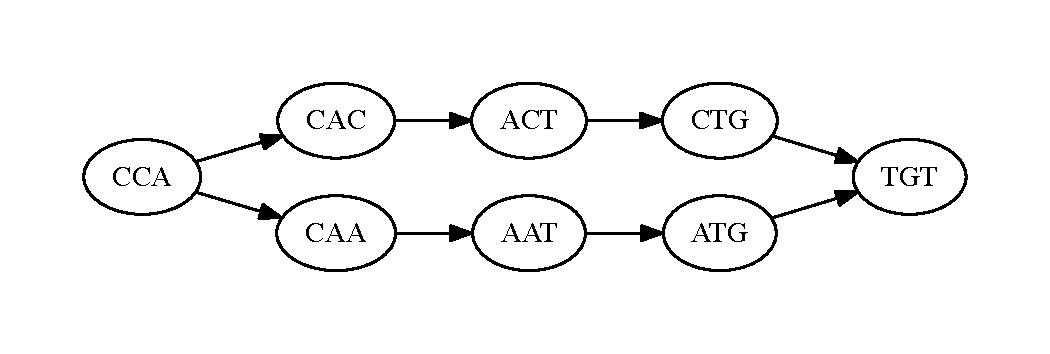
\includegraphics[width=0.95\linewidth, clip=true, trim=0 39 0 39]{graphs/sne.pdf}
\end{center}
\caption{Subgraph Corresponding To a Single Nucleotide Edit}
\label{fig:sne}
\end{figure}

If $m_i = k - 1, m_j \ge k$ or vice versa, we have a canonical INDEL edit (for convenience, we assume
that $\mathcal{S}_i'$ contains the $k - 1$ length path). Here, we can prove that there is a $m_j - m_i$
length insertion\footnote{This is equivalently an $m_j - m_i$ length deletion in $\mathcal{S}_i'$ relative to
$\mathcal{S}_j'$.} in $\mathcal{S}_j'$ relative to $\mathcal{S}_i'$, $k - 1$ letters \emph{after}
$\text{index}(s_1)$:

\begin{lemma}[Distance between $k$ length subsequences]
\label{lem:minimum-distance}
\emph{Indexed de Bruijn} graphs naturally provide a distance metric for $k$ length substrings. Let us construct an
indexed de Bruijn graph $G$ with $k$-mers of length $k$ from a non-repetitive sequence $\mathcal{S}$.
For any two $k$-mers $s_a, s_b \in \mathcal{S}, s_a \ne s_b$, the
$\text{distance}_\mathcal{S}(s_a, s_b)$ metric is equal to $l_p + 1$, where $l_p$ is the length of the
path (in $k$-mers) between $s_a$ and $s_b$. Thus, $k$-mers with overlap of $k - 1$ have an edge
directly between each other ($l_p = 0$) and a distance metric of 1. Conversely, two $k$-mers that are
adjacent but not overlapping in $\mathcal{S}$ have a distance metric of $k$, which implies $l_p = k - 1$.
\end{lemma}

\begin{proof}[Proof regarding Canonical INDELs]
\label{proof:canonical-indels}
We are given a graph $G$ which is constructed from two non-repetitive sequences $\mathcal{S}_i'$ and
$\mathcal{S}_j'$, where the only two $k$-mers in both $\mathcal{S}_i'$ and $\mathcal{S}_j'$ are $s_1$
and $s_2$ and both sequences provide independent paths between $s_1$ and $s_2$. By
Lemma~\ref{lem:minimum-distance}, if the path from $s_1 \rightarrow \dots \rightarrow s_2 \in
\mathcal{S}_i'$ has length $k - 1$, then $\mathcal{S}_i'$ is a string of length $2k$ that is formed by
concatenating $s_1, s_2$. Now, let us suppose that the path from $s_1 \rightarrow \dots \rightarrow s_2
\in \mathcal{S}_j'$ has length $k + l - 1$. The first $l$ $k$-mers after $s_1$ will introduce a $l$ length
subsequence $\mathcal{L} \subset \mathcal{S}_j', \mathcal{L} \not\subset \mathcal{S}_i'$, and then the
remaining $k - 1$ $k$-mers in the path provide a transition from $\mathcal{L}$ to $s_2$. Therefore,
$\mathcal{S}_j'$ has length of $2k + l$, and is constructed by concatenating $s_1, \mathcal{L}, s_2$.
This provides a canonical placement for the inserted sequence $\mathcal{L}$ in $\mathcal{S}_j'$ between
$s_1$ and $s_2$.
\end{proof}

To visualize the graph corresponding to a canonical INDEL, take the two example sequences
\texttt{CACTGT} and \texttt{CACCATGT}. Here, we have a \texttt{CA} insertion after position two. With
$k$-mer length $k = 3$, this corresponds to the graph in Figure~\ref{fig:indel}.

\begin{figure}[h]
\begin{center}
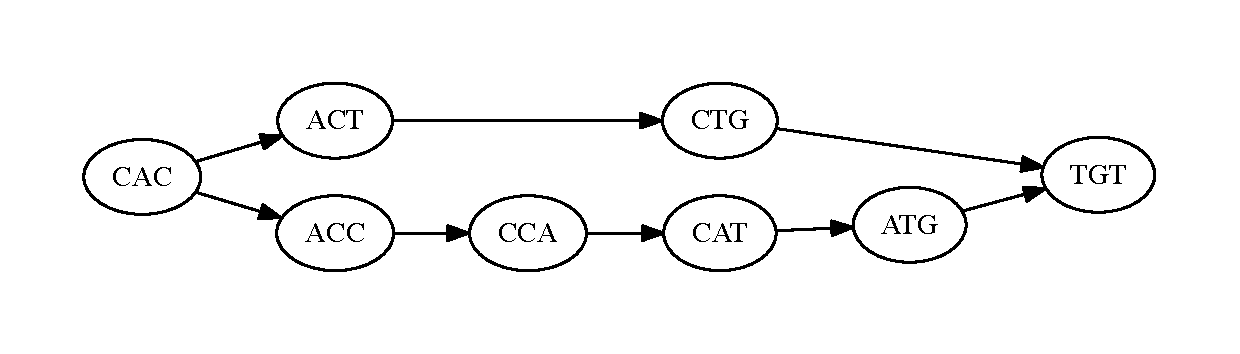
\includegraphics[width=0.95\linewidth, clip=true, trim=0 39 0 39]{graphs/indel.pdf}
\end{center}
\caption{Subgraph Corresponding To a Canonical INDEL Edit}
\label{fig:indel}
\end{figure}

Where we have a canonical allele, the cost of computing the edit is set by the need to walk the graph
linearly from $s_1$ to $s_2$, and is therefore $\mathcal{O}(n)$. However, in practice, we will see
differences that cannot be described as one of the earlier two canonical approaches. First, let us
generalize from the two above proofs: if we have two independent paths between $s_1, s_2$ in the
de Bruijn graph $G$ that was constructed from $\mathcal{S}_i, \mathcal{S}_j$, we can describe
$\mathcal{S}_i$ as a sequence created by concatenating $s_1, \mathcal{L}_i, s_2$.\footnote{This
property holds true for $\mathcal{S}_j$ as well.} The canonical edits merely result from special cases:

\begin{itemize}
\item In a canonical substitution edit, $l_{\mathcal{L}_i} = l_{\mathcal{L}_j} = 1$.
\item In a canonical INDEL edit, $l_{\mathcal{L}_i} = 0, l_{\mathcal{L}_j} \ge 1$.
\end{itemize}

Conceptually, a non-canonical edit occurs when two edits occur within $k$ positions of each other. In
this case, we can trivially fall back on a $O(nm)$ local alignment algorithm~(e.g., a pairwise HMM or
Smith-Waterman, see Durbin et al~\cite{durbin98} or Smith and Waterman~\cite{smith81}), \emph{but} we only need to locally realign
$\mathcal{L}_i$ against $\mathcal{L}_j$, which reduces the size of the realignment problem. However, we
can further limit this bound by limiting the maximum number of INDEL edits to $d = | l_{\mathcal{L}_i} -
l_{\mathcal{L}_j} |$. This allows us to use an alignment algorithm that limits the number of INDEL
edits~(e.g., Ukkonen's algorithm~\cite{ukkonen85}). By this, we can achieve $O(n(d + 1))$ cost.
Alternatively, we can decide to not further canonicalize the site, and to express it as a combined
insertion and deletion. For simplicity and performance, we use this approach in \textsc{Avocado}.

\subsection{Implementation}
\label{sec:implementation}

As alluded to earlier in this section, we can use this indexed de Bruijn concept
to canonicalize INDEL variants without needing to first build a de Bruijn graph.
The insight behind this observation is simple: any section of a read alignment
that is an exact sequence match with length greater than our $k$-mer length maps
to a section of the indexed de Bruijn graph where the read and reference paths
have converged. As such, we can use these segments that are perfect sequence
matches to anchor the bubbles containing variants (areas where the read and
reference paths through the graph diverge) without first building a graph.
We can perform this process simply by parsing the CIGAR string~(and MD tags)
for each read~\cite{li09}. We do this by:

\begin{itemize}
\item Iterating over each operator in the CIGAR string. We coalesce the operators
into a structure that we call an ``alignment block'':
\begin{itemize}
\item If the operator is a sequence match~(CIGAR \texttt{=}, or CIGAR \texttt{M}
with MD tag indicating an exact sequence match) that is longer than our $k$-mer
length, we can create an alignment block that indicates a convergence in the
indexed de Bruijn block~(a sequence match block).
\item If the sequence match operator is adjacent to an operator that indicates
that the read diverges from the reference~(insertion, deletion, or sequence
mismatch), we then take $k$ bases from the start/end of the matching sequence
and append/prepend the $k$ bases to the divergent sequence. We then create an
alignment block that indicates that the read and reference diverge, along with
the two diverging sequences, flanked by $k$ bases of matching sequence on
each side. We call these blocks realignment blocks.
\end{itemize}
\item We then loop over each alignment block. Since the sequence match blocks
are exact sequence matches, they do not need any further processing and can be
directly emitted as a CIGAR \texttt{=} operator. If the block is a realignment
block, we then apply the observations from~\S\ref{sec:formulation}. Again, we
can apply our approaches without building de Bruijn graphs for the bubble.
Specifically, both of the canonical placement rules that we formulate
in~\S\ref{sec:formulation} indicate that the variant in a bubble can be recovered
by trimming any matching flanking sequence. We begin by trimming the matching
sequences from the reference and read, starting from the right, followed
by the left. We then emit a CIGAR insertion, deletion, or sequence
mismatch~(\texttt{X}) operator for this block, along with a match operator if
either side of the flanking sequence was longer than $k$.
\end{itemize}

This process is very efficient, as it can be done wholly with standard string
operators in a single loop over the read. To avoid the cost of looking up the
reference sequence from a reference genome, we require that all reads are
tagged with the SAM \texttt{MD} tag. This allows us to reconstruct the
reference sequence for a bubble from the read sequence and CIGAR.

One problem with this method is that it can be misled by sequencing errors
that are proximal to a true variant. As can be seen in~\S\ref{sec:accuracy},
solely using our indexed de Bruijn algorithm to clean up INDEL alignments leads
to lower accuracy than the state-of-the-art toolkit. However, if the INDEL
variant in a read that is discovered is a true variant, it is a good candidate
to be used as an input to a local realignment scheme.  To implement this
approach, we used our indexed de Bruijn algorithm to canonicalize INDEL variants,
and then we used our variant discovery algorithm~(see~\S\ref{sec:discovery})
with filtration disabled to collect all canonical INDELs. We then fed these
INDELs and our input reads into \textsc{ADAM}'s INDEL realignment
engine~\cite{massie13, nothaft15}. This tool is based on the algorithms used in
the \texttt{GATK}'s INDEL realigner~\cite{depristo11}, and calculates the quality-score
weighted Hamming edit distance between a set of reads, a consensus sequence~(a
haplotype containing a potential INDEL variant), and the reference sequence. If
the sum weighted edit distance between the reads and the consensus sequence
represents a suffient improvement over the sum weighted edit distance between
the reads and the reference genome, the read alignments are moved to their
lowest weighted edit distance position relative to the consensus sequence.
A detailed description of this algorithm can be found in~\S\ref{sec:indel-realignment-implementation}.
As seen in~\S\ref{sec:accuracy}, coupling local realignment with our INDEL
canonicalization scheme improves SNP calling accuracy to comparable with the
state-of-the-art, while improving INDEL calling accuracy by 2--5\%.

\section{Genotyping}
\label{sec:genotyping}

\textsc{Avocado} performs genotyping as a several stage process where variants
are discovered from the input reads and filtered, joined back against the input
reads, and then scored. We use a biallelic likelihood model to score
variants~\cite{li11}, and run all stages in parallel. Our approach does not
rely on the input reads being sorted, and as such, is not unduly impacted by
variations in coverage across the genome. This point is critical in a parallel
approach, as coverage can vary dramatically across the genome~\cite{pinard06}.
If the input reads must be sorted, this can lead to large work imbalances
between nodes in a distributed system, which negatively impacts strong scaling.
An alternative approach is to use previously known data about genome coverage
to statically partition tasks into balanced chunks~\cite{chiang15}. Unlike the
static partitioning approach used by \textsc{SpeedSeq} that discards regions with
very high coverage, this allows us to call variants in regions with very high
coverage. However, as is also noted in the \textsc{SpeedSeq} paper, variant calls
in these regions are likely to be caused by artifacts in the reference genome that
confound mapping and thus are uninformative or spurious, and are hard filtered by
our pipeline~(see~\S\ref{sec:variant-filtration}).

\subsection{Variant Discovery and Overlapping}
\label{sec:discovery}

To identify a set of variants to score, we scan over all of the input reads,
and generate a set of variants per read where each variant is tagged with the
mean quality score of all bases in the read that were in this variant. We then
use \textsc{Apache Spark}'s \texttt{reduceByKey} functionality to compute
the number of times each variant was observed with high quality. We do this
to discard sequence variants that were observed in a read that represent a
sequencing error, and not a true variant. In our evaluation, we set the quality
needed to consider a variant observation as high quality to Phred 18~(equivalent
to a error probability of less than 0.016), and we require that a variant is
seen in at least 3 reads.

To score the discovered variants, we use an ``overlap join'' primitive to
find all of the variants that a single read overlaps. An overlap join is a
relational join where the row equality function is defined as whether two
objects overlap in the genomic coordinate space~\cite{nothaft15}. This
primitive can be implemented in a distributed system as both a broadcast
join~(the smaller of the two datasets is sent to every node in the cluster),
or as a sort-merge join, where the dataset is sorted. Our implementation
uses a broadcast strategy, as the set of variants to score is typically small
and this approach eliminates the work imbalance problem introduced earlier.

Our broadcast overlap join implementation starts by sorting the candidate
variants by genomic locus. We collect the variants to the leader node, and
then broadcast a sorted array of variants to each node in the cluster. To
find all of the variants that overlap a single read, we run a binary search
across the sorted array of variants. We prefer this strategy to building
an indexed datastructure (such as an interval tree, see Kozanitis and Patterson~\cite{kozanitis16})
because sorting can be efficiently parallelized across the \textsc{Apache
Spark} cluster, while building an indexed structure would typically need to be
done sequentially on a single node. Additionally, a flat array of sorted
variants is simpler to serialize and broadcast across the cluster than an
indexed structure. When we query into the sorted array using binary search,
the binary search algorithm will give us a variant that is overlapped by
the read. Since we actually want to run a combined join-and-group query,
we then search outwards from this first hit to identify all of the variants
that overlap the read alignment.

One of the reasons that we filter out variant sites that are not supported
by many high quality reads is an engineering limitation currently in
\textsc{Avocado}. As we decrease the stringency of the filters and allow
more variants to be detected, we increase the amount of variants that we
need to broadcast between nodes. This causes the size of data that we
must serialize to grow beyond the size of the maximum individual item
that we can serialize (limited to 2GB due to the Java Virtual Machine, which
is used by Apache Spark).
We are working to eliminate this limitation. There are several possible
strategies. A simple strategy would be to reduce the amount of data written
to the serialization buffer by compressing the data before streaming it
into the serialization buffer. However, our sorted array currently
stores the genomic coordinate of a variant separately from the variant
itself, which causes a minor amount of data duplication in memory. By
eliminating this data duplication, we should be able to eliminate this
engineering constraint.

\subsection{Genotyping Model}
\label{sec:genotyping-model}

Once we have joined our reads against our variants, we score each read using
the biallelic genotyping model proposed by Li~\cite{li11}. For each variant, we
check to see if the variant allele is present in the read at the appropriate
position in the alignment. If the variant is present, we treat the read as positive
evidence supporting the variant. If the read contains the reference allele at
that site, we treat the read as evidence supporting the reference. If the read
neither matches the variant allele nor the reference, we do not use the read
to calculate the genotype likelihoods, but we do use the read to compute
statistics~(e.g., for calculating depth, strand bias, etc.) about the genotyped
site. We calculate the genotype likelihood for the genotype in log space, using
Equation~\eqref{eq:genotype-likelihood}. Equation~\eqref{eq:genotype-likelihood}
is not our contribution and is reproduced from Li~\cite{li11}, but in log space.

\begin{align}
\label{eq:genotype-likelihood}
\log \mathcal{L}(g) &= -m k \sum_{i = 0}{j} l_r(g, m - g, \epsilon_i) \sum_{i = j + 1}^k l_r(m - g, g, \epsilon_i) \\
l_r(c_r, c_a, \epsilon) &= \text{logsum}(\log c_r + \log \epsilon, \log c_a + \text{logm1}(\log \epsilon))
\end{align}

In Equation~\eqref{eq:genotype-likelihood}, $g$ is the genotype state~(number of
reference alleles), $m$ is the copy number at the site, $k$ is the total number of
reads, $j$ is the number of reads that match the reference genome, and $\epsilon$
is the error probability of a single read base, as given by the harmonic mean of the
read's base quality, and the read's mapping quality, if present. The logsum function
adds two numbers that are in log space, while logm1 computes the additive inverse of
a number in log space. These functions can be implemented efficiently while preserving
numerical stability~\cite{durbin98}. By doing this whole calculation in log space,
we can eliminate issues caused by floating-point underflow. Additionally, since
$\epsilon$ is derived from Phred scaled quantities and is thus already in log
space (base ten), while $g$ and $m - g$ are constants that can be pre-converted to
log space. For all sites, we also compute a reference model that can be used in
joint genotyping in a gVCF approach. Additionally, we support a gVCF mode where all
sites are scored, even if they are not covered by a putative variant.

We compute the likelihoods for each read in parallel. This function maps over all
of the reads, and emits a set of records describing each observation. In addition
to storing the likelihood vector per read/variant pair, this record contains data
necessary to compute several genotype annotations that are used for variant
filtration~(such as strand bias observations, mapping quality, etc.,
see~\S\ref{sec:variant-filtration}). We use \textsc{Apache Spark}'s
\texttt{reduceByKey} function to merge all of the observations for a given
locus. Once we have merged all of the observations for a given site, we call the
genotype state by taking the genotype state with the highest likelihood. In single
sample mode, we assume no prior probability. We support a joint variant calling
mode that computes reference allele frequency for use in a binomial prior
probability distribution.

\subsection{Variant Filtration}
\label{sec:variant-filtration}

Once we have called variants, we pass the calls through a hard filtering engine.
First, unless we are in gVCF mode, we discard all homozygous reference calls and
low quality genotype calls (default threshold is Phred 30). Additionally, we
provide several hard filters that retain the genotype call, but mark the call as
filtered. These include:

\begin{enumerate}
\item Quality by depth: the Phred scaled genotype quality divided by the depth at
the site. Default value is 2.0 for heterozygous variants, 1.0 for homozygous
variants. The value can be set separately for INDELs and SNPs.
\item Root-mean-square mapping quality: Default value is 30.0 for SNPs. By default,
this filter is disabled for INDELs.
\item Depth: We filter out genotype calls below a minimum depth, or above a maximum
depth. By default, the minimum depth is 10, and maximum depth is 200. This value
can be set separately for INDELs and SNPs.
\end{enumerate}

Currently, we do not support filtering variant sites in joint genotyping mode.
However, we will add this functionality soon.

\part{Evaluation}

\chapter{Benchmarking the \textsc{ADAM} Stack}
\label{chap:benchmarking}

\chapter{The Simons Genome Diversity Dataset Recompute}
\label{chap:sgdd}

\part{Conclusion and Future Work}

\chapter{Future Work}
\label{sec:future-work}

\begin{itemize}
\item What were our overarching the goals?
  \begin{itemize}
  \item Make genomic analysis easier to scale
  \item Improve variant calling accuracy
  \item Make genomic data analysis faster
  \end{itemize}
\item Several future directions:
  \begin{itemize}
  \item Further improving query performance in \textsc{ADAM}
  \item Extending variant calling algorithms in \textsc{Avocado}
  \item Hardware acceleration for genomics
  \end{itemize}
\end{itemize}

\section{Further Query Optimization in \textsc{ADAM}}
\label{sec:extensions-adam}

\begin{itemize}
\item Preserving sorted knowledge in \textsc{ADAM}
  \begin{itemize}
  \item Needed to improve performance of region joins
  \item Currently implemented, but refactoring to extend to legacy genomic datatypes
  \item Store sorted state as metadata in the GenomicRDD.
  \end{itemize}
\item Extending what transformations can be optimized by partitioning:
  \begin{itemize}
  \item Currently just accelerate joins
  \item Aggregation queries naturally fall out of this as well
  \end{itemize}
\item Exposing other primitives as well:
  \begin{itemize}
  \item Convex hull merge
  \end{itemize}
\end{itemize}

\section{Extensions to \textsc{Avocado}}
\label{sec:extending-avocado}

\begin{itemize}
\item Deep learning for variant calling:
  \begin{itemize}
  \item Current model for INDEL discovery is intolerant of read errors
  \item Doesn't model error distribution over technologies
  \item Google \textsc{DeepVariant} uses deep learning but in an unglamorous way
  \item Would the \textsc{Avocado} INDEL canonicalization algorithm be a better fit?
  \end{itemize}
\item Somatic variant calling:
  \begin{itemize}
  \item \textsc{Avocado} currently only models a sample with known ploidy
  \item Can we accomodiate pooled or somatic variant calling?
  \item WIP towards porting over MuTect
  \end{itemize}
\end{itemize}

\section{Hardware Acceleration for Genomic Data Processing}
\label{sec:genomic-hardware}

\begin{itemize}
\item With improved I/O, single thread performance remains an issue
  \begin{itemize}
  \item As seen with \textsc{Cannoli}, hard to outperform C++ from Java
  \item However, marginal benefit to jumping to C++ is unclear
  \item Can we go directly to hardware?
  \end{itemize}
\item WIP on Genie library
\item How can we make this even more accessible?
  \begin{itemize}
  \item SQL as target language is a great opportunity
  \item Integrate Genie with Apache Arrow
  \item Allow generation of FPGA from Spark SQL plan
  \end{itemize}
\item How can we easily accomodate UDFs?
\end{itemize}

\chapter{Conclusion}
\label{chap:conclusion}

\backmatter

\bibliographystyle{abbrv}
\bibliography{fnothaft-phd-thesis}

\end{document}
